%%%%%%%%%%%%%%%%%%%%%%%%%%%%%%%%%%%%%%%%%%%%%%%%%%

% Latex Kapitel erstellen. 
% 		Kopiere 'texPandoc/*.tex' nach 'content/tex' 
% 		'content/tex' **Handarbeit... für opt. Ergebnisse!** 
% 		Kopiere 'archiv/inhalt.tex' nach 'content/' 
% 		make -- Latex-PDF erstellen 
% ju 06-Jun-2022 inhalt.tex

%%%%%%%%%%%%%%%%%%%%%%%%%%%%%%%%%%%%%%%%%%%%%%%%%%

% content/

\chapter{01-Kostenrechnung}
%%ju 16-Mai-22 01-Kostenrechnung.tex
\textbf{Kosten- und Leistungsrechnung} (KLR) $\to$ internes
Rechnungswesen

vs.

\textbf{Buchhaltung} (FiBu) $\to$ externes Rechnungswesen

\textbf{Kosten einteilen}

\begin{itemize}
\item
  Teilkosten: fixe und variable Kosten
\item
  Vollkosten: Einzelkosten und Gemeinkosten
\end{itemize}

\section{Vollkostenrechnung}\label{vollkostenrechnung}

Vgl. Kostenrechnung Fachbuch S. 79-102
(\textcite{heiser:2017:betriebsfuhrung}).

\begin{enumerate}
\item
  \textbf{Einzelkosten} (EK), direkte Kosten (Kunden), Fertigungslöhne
  $\to$ produktive Löhne

  \begin{itemize}
  \item
    \begin{enumerate}
    \def\labelenumii{\alph{enumii}.}
    \setcounter{enumii}{25}
    \item
      B. Fertigungslöhne, Anschaffungskosten, Fertigungsmaterialien
      (Ersatzteile)
    \end{enumerate}
  \item
    $\boxed{\text{FL} = WSL \cdot Flh}$\\
  \item
    (WSL) = (StLs) Werkstattschnittlohn = Stundenlohnsatz
  \end{itemize}
\item
  \textbf{Gemeinkosten} (GK), indirekte Kosten, Hilfslöhne (W-Aufträge)
  $\to$ unproduktive Löhne

  \begin{itemize}
  \item
    \begin{enumerate}
    \def\labelenumii{\alph{enumii}.}
    \setcounter{enumii}{25}
    \item
      B. Reisekosten, Kfz-Aufwendungen, Abschreibungen,
      Zinsaufwendungen, Eigenkapital-Verzinsung (kalkulatorisch)
    \end{enumerate}
  \item
    $\boxed{\text{GK} = Seko - EK} \quad \boxed{\text{GK} = \frac{WSL \cdot GKZs}{100}}$\\
  \end{itemize}
\item
  \textbf{Gemeinkostenzuschlagsatz} (GKZs) in \%

  \begin{itemize}
  \item
    $\boxed{\text{GKZs} = \frac{GK \cdot 100}{FL}}$\\
  \end{itemize}
\item
  \textbf{Kalkulatorische Kosten} Gemeinkosten, die keine Ausgaben
  verursachen; aufwandsfremde Kosten

  \begin{itemize}
  \item
    \begin{enumerate}
    \def\labelenumii{\alph{enumii}.}
    \setcounter{enumii}{25}
    \item
      B. Kalk.-Miete, Kalk.-Abschreibungen, Kalk.-Zinsen, Kalk.-U-Lohn,
      Kalk.-Wagnisse
    \end{enumerate}
  \end{itemize}
\item
  \textbf{Gewinn} (GW) in € Einkommen des Unternehmers, Wagnis,
  Unternehmensrisiko

  \begin{itemize}
  \item
    $\boxed{\text{Gewinn} = UE - EK - GK} \quad \boxed{\text{Gewinn/h} = StVs - Seko/h}$
  \end{itemize}
\item
  \textbf{Gewinnzuschlag} (GWZs) in \%

  \begin{itemize}
  \item
    $\boxed{\text{GWZs} = \frac{GW \cdot 100}{SeKo}}$
  \end{itemize}
\item
  \textbf{Umsatzerlöse, Erlöse} (UE in EUR), Stundenverrechnungssatz
  (StVs in EUR/h)

  \begin{itemize}
  \item
    Betrag für eine Lesitung = Kostendecken + Gewinn
  \item
    $\boxed{UE = EK + GK + GW} \quad \boxed{UE = Seko + GW}$
    (Selbstkosten + Gewinn)
  \item
    $\boxed{StVs = StLs/WSL + GK + GW}$
  \end{itemize}
\item
  \textbf{Selbstkosten} (SeKo)

  \begin{itemize}
  \item
    $\boxed{SeKo = EK + GK}$ (Einzelkosten + Gemeinkosten)
  \item
    $\boxed{SeKo = FL + GK}$ vs.~$\boxed{SeKo/h = WSL + GK/h}$
  \item
    $\boxed{SeKo_{EUR} = UE - GW} \to \boxed{SeKo_\% = 100~\% - UR_\%}$
  \end{itemize}
\end{enumerate}

\begin{figure}[!ht]% hier: !ht
\centering
\includegraphics[width=0.4\textwidth]{images/Skizze/02_Umsatzerloese_Skizze.pdf}
\caption{Kosten und Erlöse}
%\label{fig:}%% anpassen
\end{figure}

\newpage

\subsection{Kosten der Werkstatt}\label{kosten-der-werkstatt}

\begin{enumerate}
\item
  \textbf{Fertigungslöhne} (FL), >>produktiv<<, EK, direkt

  \begin{itemize}
  \item
    Auftrag direkt dem Kunden in Rechnung stellen
  \item
    $\boxed{\text{FL} = WSL \cdot Flh}$
  \item
    \begin{enumerate}
    \def\labelenumii{\alph{enumii}.}
    \setcounter{enumii}{25}
    \item
      B. $90~\%$ Lohnkosten
    \end{enumerate}
  \end{itemize}
\end{enumerate}

$+$

\begin{enumerate}
\setcounter{enumi}{1}
\item
  \textbf{Hilfslöhne} (HL) >>unproduktiv<<, GK, nicht direkt, entstehen
  bei Werkstattaufträgen

  \begin{itemize}
  \item
    W-Aufträge z. B. Leerlauf, Nacharbeiten, Reparatur von
    Werkstattfahrzeuge, Urlaub, Feiertage, Wartezeiten
  \item
    \begin{enumerate}
    \def\labelenumii{\alph{enumii}.}
    \setcounter{enumii}{25}
    \item
      B. $10~\%$ Lohnkosten
    \end{enumerate}
  \end{itemize}
\end{enumerate}

$= 100~\%$

\textbf{Fertigungslöhne entstehen bei}

\begin{enumerate}
\item
  \textbf{K-Aufträge}

  \begin{itemize}
  \item
    Kundenauftrag, externe Aufträge
  \item
    \begin{enumerate}
    \def\labelenumii{\alph{enumii}.}
    \setcounter{enumii}{25}
    \item
      B. Wartung, Kundendienst, Reparatur
    \end{enumerate}
  \end{itemize}
\item
  \textbf{I-Aufträge}

  \begin{itemize}
  \item
    interne Aufträge, innerbetrieblich (andere Abteilung des Betriebs)
  \item
    \begin{enumerate}
    \def\labelenumii{\alph{enumii}.}
    \setcounter{enumii}{25}
    \item
      B. Fahrzeugaufbereitung, Gebrauchtwagenreparatur, Überführung,
      Übergabedurchsicht
    \end{enumerate}
  \end{itemize}
\item
  \textbf{G+K-Aufträge}

  \begin{itemize}
  \item
    Garantie- und Kulanzanträge
  \item
    für Kunden ohne Berechnung, Gründe: Kulanz, Sachmängelhaftung,
    Kundenzufriedenheit gewährleisten
  \end{itemize}
\end{enumerate}

\textbf{Zeitlohn vs.~Leistungslohn}

\begin{enumerate}
\item
  \textbf{FL - Zeitlohn} Fertigungslohn, produktive Arbeitszeit,
  Stundenlohn

  \begin{itemize}
  \item
    \textbf{FLh} Fertigungslohnstunden
  \item
    \textbf{WSL} Werkstattschnittlohn, quer durch die Werkstatt z. B.
    Lehrling, Geselle

    \begin{itemize}
    \item
      $\boxed{\text{WSL} = \frac{FL}{Flh}}$
    \end{itemize}
  \item
    \textbf{MAZ} Mehrarbeitszuschlag
  \end{itemize}
\item
  \textbf{FL - Leistungslohn} Lohn für die erbrachte Leistung

  \begin{itemize}
  \item
    \textbf{AWLs} Arbeitswertlohnsatz
  \item
    \textbf{ZELs} Zeiteinheitenlohnsatz
  \item
    \textbf{Soll-AW} Vorgabe, wie viele AW muss ich in einer Stunde
    machen?
  \item
    \textbf{Ist-AW} tatsächlich erbrachte Leistung
  \item
    \textbf{Mehr-AW} Mehrleistung in AW
    $\boxed{\text{AW} = \text{Ist-AW} - \text{Soll-AW}}$
  \end{itemize}
\end{enumerate}

\textbf{Vorgabezeiten} Grundlage für Leistungslohn

\begin{itemize}
\item
  \textbf{ZE} Zeiteinheit (in Min.)

  \begin{itemize}
  \item
    (StVs / 60 = €/ZE x Min. = Preis (€))
  \end{itemize}
\item
  \textbf{AW} Arbeitswert (in Min.) Richtzeiten, Vorgabezeiten
\item
  \textbf{WF} Werkstattfaktor $\to$ wie viele AW/ZE in einer Stunde?
  (Soll-Leistung, Mindestleistung)

  \begin{itemize}
  \item
    (12 AW/h = $\frac{60}{12}$ alle 5 Min. 1 AW)
  \end{itemize}
\item
  \textbf{LF} Leistungsfaktor (Ist-Leistung)
\end{itemize}

\newpage

\subsection{Kennwerte der Werkstatt}\label{kennwerte-der-werkstatt}

\begin{enumerate}
\item
  \textbf{Soll-Umsatzerlös} (Soll-UE) deckt die Selbstkosten ab

  \begin{itemize}
  \item
    Soll-UE = Seko + GW
  \end{itemize}
\item
  \textbf{Ist-Umsatzerlös} tatsächlich erwirtschaftete Umsatz
\item
  \textbf{Lohnerlöse} Umsatzerlöse
\item
  \textbf{Wirtschaftlichkeit} (WI) wurde Gewinn oder Verlust gemacht z.
  B. 1,05 \% $\to$ 5 \% mehr

  \begin{itemize}
  \item
    Wirtschaftlichkeit = Umsatzerlöse / Selbstkosten
  \item
    WI = LE / Seko; WI = UE/Seko
  \item
    WI > 1 Gewinn
  \item
    WI \textless{} 1 Verlust
  \item
    WI = 1 Kostendeckend
  \end{itemize}
\item
  \textbf{Produktivität} (PR)

  \begin{itemize}
  \item
    Gesamte Arbeitszeit (Fertigungs- + Hilfslohnstunden)
  \item
    Produktivität = Fertigungslohnstunden x 100 / Arbeitszeit
  \item
    PR = FLh x 100 / AZ\\
  \end{itemize}
\item
  \textbf{Leistungsfaktor} (LF)

  \begin{itemize}
  \item
    tatsächlich erbrachte Leistung je Stunde
  \item
    Leistungsfaktor = Ist-Leistung in AW / Fertigungslohnstunden
  \item
    LF = Ist-AW / FLh
  \end{itemize}
\item
  \textbf{Leistungsgrad} (LG)

  \begin{itemize}
  \item
    $\boxed{\text{LG} = \frac{\text{Ist-AW}}{\text{Soll-AW}}}$
  \item
    (Ist-Leistung / Soll-Leistung) und (tatsächlich erbrachte Leistung /
    Mindestleistung)
  \end{itemize}
\item
  \textbf{Leistungslohnsatz}

  \begin{itemize}
  \item
    Leistungslohnsatz = Fertigungslohn / Fertigungslohnstunden
  \item
    LLs = FL / FLh
  \end{itemize}
\item
  \textbf{Umsatzrentabilität} (UR) in \%
\end{enumerate}

\begin{itemize}
\item
  Wie viel Prozent des Umsatzes als Gewinn anfallen
\item
  $\boxed{\text{UR} = \frac{GW \cdot 100}{UE}} \quad \boxed{\text{UR} = \frac{GW/h \cdot 100}{StVs}}$
\end{itemize}

\subsubsection{Kostenindex - Stundenverrechnungssatz - AW-Vs
(Prüfung)}\label{kostenindex-stundenverrechnungssatz-aw-vs-pruefung}

\emph{3x wichtige Formeln}

\textbf{Kostenindex, Werkstattindex, Faktor} (KI) wievielmal mehr der
Kunde für eine Fertigungslohnstunde zu bezahlen hat, als der Monteur in
dieser Stunde verdient. (bezieht sich auf Löhne)

$\boxed{\text{KI} = \frac{\text{Prod. Löhne} + \text{GK} + \text{Gewinn}}{\text{Prod. Löhne}}} \quad$
$\boxed{\text{KI} = \frac{\text{StVs}}{\text{WSL}}} \quad \boxed{\text{KI} = \frac{\text{UE}}{\text{FL}}}$

\textbf{Stundenverrechnungssatz} Arbeitspreis, der dem Kunden für eine
Stunde berechnet wird. Reparaturstunde = Fertigungslohnstunde

$\boxed{\text{StVs} = \frac{\text{UE}}{\text{FLh}}} \quad \boxed{\text{StVs} = \text{KI} \cdot \text{WSL}}$

$\boxed{\text{StVs}_{neu} = \frac{\text{Seko}_{neu} \cdot 100~\%}{\text{Seko}_{alt}}} \quad \boxed{\Delta \text{StVs} = \text{StVs}_{neu} - \text{StVs}_{alt}}$

Erhöhung
$\boxed{\text{StVs}_\% = \frac{\Delta \text{StVs} \cdot 100~\%}{\text{StVs}_{alt}}}$

\textbf{AW-Verrechnungssatz} Ermittlung des Arbeitspreises für eine
Arbeitsposition (Leistungslohn)

Erlös je AW

$\boxed{\text{AW-Vs} = \frac{\text{StVs}}{\text{WF}}} \quad \boxed{\text{AW-Vs} = \frac{\text{WSL} \cdot \text{KI}}{\text{WF}}} \quad \boxed{\text{AW-Vs} = \frac{\text{UE}}{\text{FLh} \cdot \text{WF}}}$

\subsubsection{Reparaturkosten
berechnen}\label{reparaturkosten-berechnen}

\textbf{Rechnungserstellung - Formvorschriften beachten}

\begin{itemize}
\item
  Rechnung schriftlich mit Rechnungsnummer und Leistungsdatum
\item
  Kunden- und Fahrzeugdaten wichtige aufführen
\item
  Arbeitskreis und Ersatzteilpreise detailliert aufführen
\item
  Netto-Rechnungsbetrag, Umsatzsteuer, Altteilesteuer und
  Brutto-Rechnungsbetrag einzeln aufführen.
\end{itemize}

\lstset{language=Bash}% C, TeX, Bash, Python 
\begin{lstlisting}[
	%caption={}, label={code:}%% anpassen
]
  Arbeitspreis      = Flh x StVs
+ Materialkosten  
= Reparaturkosten 
+ Umsatzsteuer        19 % 
_____________________________________________
= Rechnungsbetrag                         EUR
\end{lstlisting}

\newpage

\subsection{Handelswarenkalkulation}\label{handelswarenkalkulation}

\textbf{Kalkulationsarten} Vorwärts-, Rückwärts-, Differenzkalkulation

\subsubsection{Einkaufskalkulation}\label{einkaufskalkulation}

\lstset{language=Bash}% C, TeX, Bash, Python 
\begin{lstlisting}[
	%caption={}, label={code:}%% anpassen
]
  BP                                           LEP                 // 100 %
- BK                                         - Rabatt       10 %                 
= BEP                           // 98 %      = ZEP                 // 100 % 
+ Skonto    2 % (in 100)                     - Skonto        2 %
= ZEP                           // 90 %      = BEP                 
+ Rabatt   10 % (in 100)                     + BK
________________________________             ______________________         
= LEP                           EUR          = BP                  EUR 
\end{lstlisting}

\begin{enumerate}
\item
  \textbf{Listeneinkaufspreis} (LEP), Ware, Angebot,
  $\boxed{BEP + \text{Skonto} + \text{Rabatt}}$
\item
  \textbf{Lieferantenrabatt} (LRa), Preisnachlass
\item
  \textbf{Zieleinkaufspreis} (ZEP), Zahlungszeitpunkt, Kauf auf Ziel
  $\boxed{BEP + \text{Skonto}}$
\item
  \textbf{Lieferantenskonto} (LSk)
\item
  \textbf{Bareinkaufspreis} (BEP), bei sofortiger Barzahlung
\item
  \textbf{Bezugskosten} (BK), Transport: Verpackung, Fracht, Zoll,
  Rollgeld
\end{enumerate}

\subsubsection{Verkaufskalkulation,
Ersatzteilkalkulation}\label{verkaufskalkulation-ersatzteilkalkulation}

\lstset{language=Bash}% C, TeX, Bash, Python 
\begin{lstlisting}[
	%caption={}, label={code:}%% anpassen
]
  BP                                           LVP                 // 100 %
+ GK       20 % (auf 100)                    - Rabatt       10 %                 
= SEKO                                       = ZVP                 // 100 %
+ Gewinn    8 % (auf 100)                    - Skonto        2 %
= BVP                           // 98 %      = BVP        
+ Skonto    2 % (in 100)                     - Gewinn
= ZVP                           // 90 %      = Seko                 
+ Rabatt   10 % (in 100)                     - GKZs
________________________________             ______________________          
= LVP                           EUR          = BP                  EUR
+ UST      19 %                                                 
________________________________                        
= Rechnungsbetrag ohne Rabatt   EUR                                 
\end{lstlisting}

\begin{enumerate}
\item
  \textbf{Bezugspreis} (BP), Anschaffungskosten, Einstandspreis
  $\boxed{BEP + BK}$
\item
  \textbf{Gemeinkosten} (GK), anteilig, nicht direkt
\item
  \textbf{Selbstkosten} (SEKO), Beschaffung, Bereitstellung,
  Weiterverarbeitung
\item
  \textbf{Gewinn} Wagnis, U-Lohn
\item
  \textbf{Verkaufssonderkosten} Garantie, Provision, Kundendienst
\item
  \textbf{Barverkaufspreis} (BVP) $\boxed{BP + GK + \text{Gewinn}}$
\item
  \textbf{Kundenskonto} (KSk)
\item
  \textbf{Zielverkaufspreis} (ZVP)
  $\boxed{BP + GK + \text{Gewinn} + \text{Skonto}}$
\item
  \textbf{Kundenrabatt} (KRa)
\item
  \textbf{Listenverkaufspreis} (LVP)
  $\boxed{BP + GK + \text{Gewinn} + \text{Skonto} + \text{Rabatt}}$
\end{enumerate}

\subsubsection{Kalkulationsfaktor}\label{kalkulationsfaktor}

Vgl. Tabellenbuch S. 61 und 69 (\textcite{bell:2021:tabellenbuchKfz}).

\begin{figure}[!ht]% hier: !ht
\centering
\includegraphics[width=0.6\textwidth]{images/Skizze/03_Kalkulationsfaktor_Skizze.pdf}
\caption{Kalkulationsfaktor}
%\label{fig:}%% anpassen
\end{figure}

\textbf{Kalkulationsfaktor} (KF) wievielmal höher der (Verkaufspreis =
Listenpreis) gegenüber (Bezugspreis) bezieht sich auf das Lager,
Ersatzteil

$\boxed{KF = \frac{LVP}{BP}} \quad \to \boxed{LVP = BP \cdot KF}$

\textbf{Kalkulationszuschlag} enthält
$(GK + \text{Gewinn} + \text{Skonto} + \text{Rabatt})$ bezogen auf
(Bezugspreis)

\textbf{Handelsspanne} (HSP) unterschied zwischen (Verkaufspreis +
Bezugspreis) bezogen auf (Verkaufspreis)
$\boxed{HSP_\% = \frac{HSP \cdot 100}{LVP}}$
$\boxed{HSP_\text{EUR} = LVP - BP}$

\subsubsection{Verkauf von Tauschteilen und
Agenturwarenverkauf}\label{verkauf-von-tauschteilen-und-agenturwarenverkauf}

\textbf{Altteilesteuer} (AT-St) kauft ein Kunde ein Tauschteil und gibt
dabei sein defektes Teil (Altteil) in Zahlung, fällt Altteilesteuer an.
$\boxed{LVP \cdot 10~\% \cdot 19~\%}$

\textbf{Agenturwaren} sind Waren, die im Auftrag und auf Rechnung einer
Fremdfirma verkauft werden (Preise inkl. Gesetzl. Ust.).

\chapter{02-Auftragsabwicklung}
%%ju 16-Mai-22 02-Auftragsabwicklung.tex
\section{KFZ-Werkvertrag - Reparaturauftrag /
Werkstattauftrag}\label{kfz-werkvertrag-reparaturauftrag-werkstattauftrag}

\begin{itemize}
\item
  geschäftliche Beziehung zwischen >>Autohaus / Werkstatt<<
  (Auftragnehmer) und dem >>Kunde<< (Auftraggeber)
\item
  Merkmal ist die >>Auftragsnummer<<
\item
  gesetzliche Regelung (Werkvertragsrecht)

  \begin{itemize}
  \item
    \emph{§631} (BGB) Autohaus verpflichtet sich zur Reparatur, Wartung

    \begin{itemize}
    \item
      Erfolg geschuldet
    \end{itemize}
  \item
    \emph{§632} (BGB) Kunde verpflichtet sich zur Entrichtung der
    vereinbarten Vergütung, Werklohn

    \begin{itemize}
    \item
      Kunde muss zahlen, auch wenn über Preise nicht gesprochen wurde,
      aber keine Wucherpreise
    \end{itemize}
  \item
    \emph{§633 Absatz 1} (BGB) Autohaus schuldet Arbeitserfolg, trägt
    Risiko

    \begin{itemize}
    \item
      nach Reparatur oder Umbauten muss Fahrzeug benutzbar, technisch
      einwandfrei sein
    \end{itemize}
  \end{itemize}
\end{itemize}

\textbf{Wichtige Punkte - Reparaturauftrag}

\begin{itemize}
\item
  Daten vom Kunden bei Auftragsvereinbarung
\item
  alle vom Kunden in Auftrag gegebenen Arbeiten schriftlich
  dokumentieren
\item
  Kundenadresse, Telefonnummer (Erreichbarkeit)
\item
  Fahrzeugdaten

  \begin{itemize}
  \item
    Fahrzeugtyp
  \item
    Fahrzeug-Ident-Nr.
  \item
    Erstzulassung
  \item
    Zulassungsdatum
  \item
    Kennzeichen
  \item
    Kilometerstand
  \end{itemize}
\item
  Auftragsdatum
\item
  unverbindlichen Fertigstellungstermin
\item
  Zustand des Fahrzeuges (Unfallschäden), Tankinhalt
\item
  Kundenunterschrift
\end{itemize}

\textbf{Welche rechtliche Möglichkeit hat der Kunde, wenn Termin nicht
eingehalten wird?}

Der Kunde kann die Werkstatt in Verzug setzen und gegebenenfalls
Schadenersatz verlangen.

\textbf{Welche Möglichkeit hat der Kunde, wenn er einen Mangel an seinem
neuen Fahrzeug feststellt?}

Käufer hat Recht

\begin{itemize}
\item
  auf Nacherfüllung (Reparatur oder Neulieferung)
\item
  Rücktritt
\item
  Minderung des Kaufpreises
\item
  Anspruch auf Schadenersatz statt der Leistung
\item
  Ersatz vergeblicher Leistungen
\end{itemize}

\textbf{Unterschied zwischen Garantie und Sachmängelhaftung}

Garantie ist eine freiwillige Leistung des Betriebes. Die
Garantielaufzeit kann frei mit dem Kunden vereinbart werden.

Die Sachmängelhaftung ist vom Gesetzgeber vorgeschrieben und ist 24
Monate beziehungsweise mit Einschränkung 12 Monate gültig (gebrauchte
Ware).

\textbf{Beweislast im Rahmen der Sachmängelhaftung}

\begin{itemize}
\item
  bis 6 Monate: Beweislast beim Unternehmen
\item
  nach 6 Monate: Unternehmen kann Beweislast auf den Kunden umkehren
\end{itemize}

\newpage

\section{Aufträge unterteilen}\label{auftraege-unterteilen}

\begin{enumerate}
\item
  \textbf{Kundenaufträge} (K-Aufträge) z. B. Wartung, Reparatur

  \begin{itemize}
  \item
    $\to$ produktive Löhne
  \end{itemize}
\item
  \textbf{Interne Aufträge} (I-Aufträge) z. B. Gebrauchtwagenreparaturen

  \begin{itemize}
  \item
    $\to$ produktive Löhne
  \end{itemize}
\item
  \textbf{Werkstattaufträge} (W-Aufträge) z. B. Halle säubern

  \begin{itemize}
  \item
    $\to$ unproduktive Werkstattleistungen (Hilfslöhne, Gemeinkosten)
  \end{itemize}
\item
  \textbf{Garantie- und Kulanzanträge} (G+K-Aufträge) z. B. Kulanz-,
  Garantiearbeiten

  \begin{itemize}
  \item
    $\to$ produktive Löhne
  \end{itemize}
\item
  \textbf{Fremdleistungsaufträge} (FL-Aufträge) z. B. Lackierungen,
  Dellendoktor, Sattler

  \begin{itemize}
  \item
    $\to$ produktive Löhne
  \end{itemize}
\end{enumerate}

\textbf{W-Aufträge} (Werkstattaufträge)

\begin{itemize}
\item
  W1 = Allgemeine Werkstattarbeiten
\item
  W2 = Leerlaufstunden und Wartezeit
\item
  W3 = Reparaturen an Werkstatt eigenen Fahrzeugen
\item
  W4 = Nacharbeit, eigene Gewährleistung und Kulanz
\item
  W5 = Urlaub, Feiertage
\item
  W6 = Schulung
\item
  W7 = Krankheit
\end{itemize}

\textbf{Was sind produktive Löhne?}

Vgl. Fachbuch S. 172 (\textcite{heiser:2017:betriebsfuhrung}).

\begin{enumerate}
\item
  Kundenaufträge
\item
  Interne Aufträge
\item
  Garantie- und Kulanzanträge
\item
  Fremdleistungsaufträge
\end{enumerate}

\textbf{Was sind unproduktive Löhne?}

Werkstattaufträge

\newpage

\section{Arbeitszeitmodelle und
Zeitplanung}\label{arbeitszeitmodelle-und-zeitplanung}

Vgl. Arbeitszeit ermitteln Fachbuch S. 170-171
(\textcite{heiser:2017:betriebsfuhrung}).

\textbf{Arbeitszeitermittlung}

\begin{figure}[!ht]% hier: !ht
\centering
\includegraphics[width=0.9\textwidth]{images/Skizze/Arbeitszeitermittlung.pdf}
\caption{Arbeitszeitermittlung}
%\label{fig:}%% anpassen
\end{figure}

\textbf{Ermittlungsschema}

\lstset{language=Bash}% C, TeX, Bash, Python 
\begin{lstlisting}[
	%caption={}, label={code:}%% anpassen
]
  Kalendertage pro Jahr                              365
- Samstag/Sonntag (5-Tage-Woche, 52 x 2)             104
= Mögliche Arbeitszeit (Brutto)                      261
- Feiertage (je Bundesland)                            9
- Urlaubstage (min. 24 Werktage)                      29
- Krankheitstage                                       8
- Schulungstage                                        6 
= Mögliche Anwesenheitstage (Netto)                  209
  Tägliche Arbeitszeit 8 h 
_____________________________________________________________
= Mögliche Anwesenheitszeit in Stunden (209 x 8 h) 1.672 h
  Leistungszeit (produktive Arbeitszeit)
  Leerlauf      (unproduktive Arbeitszeit)
_____________________________________________________________
= Arbeitstage pro Jahr (261 - Feiertage)             252 Tage
\end{lstlisting}

\textbf{Werktag} (Mo. - Sa.)

\newpage

\section{Serviceberater - Kundendienstberater -
Dialogannahme}\label{serviceberater-kundendienstberater-dialogannahme}

\textbf{Skript - Serviceberater}

\begin{itemize}
\item
  >>Mädchen für alles<<
\item
  Vollzeitjob, hat viele Einsatzmöglichkeiten
\item
  Im Durchschnitt 8 bis 14 Kunden pro Tag
\item
  Small Talk halten: Wieso, Weshalb, Warum?
\item
  Das kleine 1x1 des Serviceberaters
\end{itemize}

\textbf{Vorgehensweise des KD-Beraters bei der Auftragsannahme}

\begin{itemize}
\item
  Fragen nach dem Kundenwunsch
\item
  Durchführung der Untersuchung des Fahrzeuges
\item
  Dokumentation von Schäden am Fahrzeug
\item
  Erfassung von Wertgegenständen im Fahrzeug
\item
  Probefahrt mit dem Kunden
\item
  Mitteilung des kalkulierten Preises
\item
  Auftrag erstellen
\end{itemize}

\textbf{Bereiche des Autohauses, die an der Bearbeitung des Auftrags
beteiligt sind?}

\begin{enumerate}
\item
  \textbf{Annahme Kundendienst}

  \begin{itemize}
  \item
    \emph{Aufgaben} Annahme von Reparaturen, technische Beratung des
    Kunden, Fahrzeugübergabe
  \end{itemize}
\item
  \textbf{Werkstatt}

  \begin{itemize}
  \item
    \emph{Aufgaben} Durchführung von Reparaturen und Wartungsarbeiten
  \end{itemize}
\item
  \textbf{Teiledienst}

  \begin{itemize}
  \item
    \emph{Aufgaben} Verwaltung von den Ersatzteilen und Zubehör, Ausgabe
    von Teilen, Verkauf von Teilen
  \end{itemize}
\item
  \textbf{Verkauf}

  \begin{itemize}
  \item
    \emph{Aufgaben} Kundenberatung
  \end{itemize}
\item
  \textbf{Verwaltung}

  \begin{itemize}
  \item
    \emph{Aufgaben} Zahlungserinnerung einer nicht gezahlten Rechnung an
    den Kunden
  \end{itemize}
\item
  \textbf{Geschäftsleitung}

  \begin{itemize}
  \item
    \emph{Aufgaben} Kundenbeschwerde über eine zu hohe Rechnung
  \end{itemize}
\end{enumerate}

\textbf{Vorteile Direktannahme}

\begin{itemize}
\item
  Möglichkeit zur Kommunikation mit dem Kunden schaffen
\item
  über Mängel sofort informieren
\item
  Missverständnisse können vermieden werden
\item
  Rückfragen werden verringert
\item
  teure Reparatur erkennen vs.~Zeitwert / Wiederbeschaffungswert $\to$
  zeitwertgerechte Reparatur
\item
  günstige Ersatzteile oder Gebrauchtteile $\to$ verkehrstüchtigen
  Zustand
\item
  bei sicherheitsrelevanten Mängel $\to$ nicht mehr fahren lassen!
  (Polizei informieren bei hartnäckigen Fällen)
\item
  Entscheidend ist kompetente Person oder Schnarchnase!
\end{itemize}

\section{Auftragsabwicklung und
Kundenservice}\label{auftragsabwicklung-und-kundenservice}

Vgl. Auftragsabwicklung Fachbuch S. 149-158
(\textcite{heiser:2017:betriebsfuhrung}).

\textbf{Arbeitsplanung - Auftragsannahme bis Fahrzeugrückgabe}

\begin{enumerate}
\item
  \textbf{Terminvereinbarung} Auftragsannahme

  \begin{itemize}
  \item
    Termin mit Kunden vereinbaren, Terminvorbereitung
  \end{itemize}
\item
  \textbf{Terminvorbereitung}

  \begin{itemize}
  \item
    KD-Berater plant Fahrzeugdurchsicht auf Basis Fahrzeughistorie
  \end{itemize}
\item
  \textbf{Fahrzeugannahme}

  \begin{itemize}
  \item
    Fahrzeug wird vom KD-Berater übernommen und Fahrzeugcheck
    durchgeführt
  \end{itemize}
\item
  \textbf{Auftragserstellung}

  \begin{itemize}
  \item
    notwendige Arbeiten erfassen und Werkstattauftrag erstellen
  \item
    Teileverfügbarkeit prüfen
  \end{itemize}
\item
  \textbf{Reparatur}

  \begin{itemize}
  \item
    In der Werkstatt wird nach Herstellervorgaben des Fahrzeug instand
    gesetzt
  \end{itemize}
\item
  \textbf{Qualitätskontrolle}

  \begin{itemize}
  \item
    Ausführung der Arbeit überprüfen, Endkontrolle / Sichtkontrolle /
    Probefahrt
  \end{itemize}
\item
  \textbf{Vorbereiten der Fahrzeugrückgabe}

  \begin{itemize}
  \item
    Rückgabe vorbereiten und Rechnung erstellen, Rechnung prüfen
  \end{itemize}
\item
  \textbf{Fahrzeugrückgabe}

  \begin{itemize}
  \item
    Fahrzeug an Kunde übergeben und Arbeiten anhand der Rechnung
    erläutern, Kunde zahlt Rechnung
  \end{itemize}
\item
  \textbf{Nachbearbeitung}

  \begin{itemize}
  \item
    Kundenzufriedenheit prüfen anhand von Nachfragen
  \item
    anonymer Fragebogen (telefonisch, Internet, Post)
  \end{itemize}
\end{enumerate}

\textbf{Organigramm} $\to$ Hierarchisch strukturiert,
Organisationsstruktur, Weisungsbeziehungen

\textbf{Softskills} $\to$ Selbstsicherheit, Selbstständigkeit,
Entscheidungsfähigkeit

\section{Betriebsorganisation}\label{betriebsorganisation}

Das Ziel ist, Gewinn zu erzielen. Dies wird erreicht durch den optimalen
Einsatz von Mitarbeitern, Maschinen, Material und Zeit.

\textbf{Maximalprinzip}: Mit gegebenen Mitteln eine möglichst hohe
Leistung erzielen. \textbf{Minimalprinzip}: Eine vorbestimmte Leistung
mit möglichst geringen Mitteln erzielen.

\textbf{Kundenorientierung} ist die Ausrichtung des Denkens und Handelns
der Mitarbeiter auf den Kunden und seine Bedürfnisse. Macht das
wirtschaftlich Sinn?

\textbf{Was beeinflusst die Kundenzufriedenheit? Nenne Merkmale}

\begin{itemize}
\item
  \textbf{Technische Produktqualität}

  \begin{itemize}
  \item
    Verarbeitung und Reparaturanfälligkeit
  \item
    Ausführung von Wartungs- und Reparaturarbeiten
  \end{itemize}
\item
  \textbf{Servicequalität}

  \begin{itemize}
  \item
    Kulanzregelungen
  \item
    Einhaltung von Terminen
  \item
    Qualität der Beratung
  \item
    Umgang mit Reklamationen an
  \end{itemize}
\item
  Reputationsqualität

  \begin{itemize}
  \item
    Guter Ruf, Kompetenz
  \end{itemize}
\item
  Persönliche Beziehungsqualität

  \begin{itemize}
  \item
    Mitarbeiter - Kunde
  \end{itemize}
\item
  Preiswahrnehmung

  \begin{itemize}
  \item
    Gutes Preis-Leistungs-Verhältnis, Angebote, Transparenz
  \end{itemize}
\item
  Kundenbindung

  \begin{itemize}
  \item
    Ziel: langfristige Bindung
  \end{itemize}
\end{itemize}

\textbf{Servicekonzepte, die Kundenbindung verbessern}

\begin{itemize}
\item
  Werbung
\item
  Garantie und Kulanz
\item
  Hol- und Bring-Service
\item
  Reparatur-Finanzierung
\item
  Dienstleistungsangebote: Verkauf, Wartung
\end{itemize}

Bestandskunden halten vs.~Neukunden bewerben kostet 5-6x mehr

\textbf{Kundenarten}

\begin{itemize}
\item
  \textbf{Laufkunde} (Kommt zufällig und hat keine Bindung)

  \begin{itemize}
  \item
    \emph{Bedeutung} Gering
  \item
    \emph{Erwartung des Kunden} Schnelle und zuverlässige Ausführung der
    Arbeit
  \item
    \emph{Maßnahmen} Keine
  \end{itemize}
\item
  \textbf{Dauerkunde} (nimmt gelegentlich Service in Anspruch)

  \begin{itemize}
  \item
    \emph{Bedeutung} Mittel
  \item
    \emph{Erwartung des Kunden} zuverlässig und preisgünstig
  \item
    \emph{Maßnahmen} Angebote an Kunden
  \end{itemize}
\item
  \textbf{Stammkunde} (lässt alle Arbeiten in der Werkstatt ausführen)

  \begin{itemize}
  \item
    \emph{Bedeutung} Hoch
  \item
    \emph{Erwartung des Kunden} persönliche Betreuung
  \item
    \emph{Maßnahmen} persönliche Ansprache
  \end{itemize}
\item
  \textbf{Großkunde} (Gesamten Fuhrpark warten)

  \begin{itemize}
  \item
    \emph{Bedeutung} sehr hoch
  \item
    \emph{Erwartung des Kunden} Schnelle und gute Ausführung, Kulanz
  \item
    \emph{Maßnahmen} Rabatt, Terminvereinbarung
  \end{itemize}
\end{itemize}

\emph{Vorsicht bei Zahlungszielen} von 30 oder 60 Tage Z. B. Aldi legt
bei einer Bank stundenweise / 28 Tage lang Geld an und lässt das Geld
für sich arbeiten.

\section{Reklamation und Umtausch}\label{reklamation-und-umtausch}

\textbf{Reklamationen} sind nicht erfüllte Kundenerwartungen

\begin{itemize}
\item
  Kundenbedürfnisse herausfinden
\item
  kundenorientierte Lösung anbieten (Kulanz bei einem guten Kunden)
\item
  bei Kundenzufriedenheit kommen Kunden wieder
\end{itemize}

\textbf{Umtausch} geht es um die Rücknahme eines fehlerfreien Produktes

\textbf{Kundenreklamation}

\begin{itemize}
\item
  \emph{Beschwerden als Chance sehen}
\item
  Reklamationsmanagement hilft bei der Kundenbindung
\item
  Beschwerden anregen (Beispiel Fragebögen)
\item
  \emph{Valide} Aussagekräftig
\item
  Wirtschaftspsychologe werten Fragebögen aus
\item
  Kontrollmechanismus einbauen -- kommt die Beschwerde auch an?
\end{itemize}

\chapter{03-Betriebsfuehrung}
%%ju 28-Mai-22 03-Betriebsfuehrung.tex
\section{Betriebsorganisation}\label{betriebsorganisation}

Ein Unternehmen ist auf die Optimierung des Gewinns ausgerichtet. Dies
wird erreicht durch den optimalen Einsatz von Mitarbeitern, Maschinen,
Material und Zeit.

\newpage

\subsection{Aufbauorganisation -- Geschäftsbereiche eines
Autohauses}\label{aufbauorganisation-geschaeftsbereiche-eines-autohauses}

\textbf{Organigramm} $\to$ Hierarchisch strukturiert,
Organisationsstruktur, Weisungsbeziehungen

\textbf{Softskills} $\to$ Selbstsicherheit, Selbstständigkeit,
Entscheidungsfähigkeit

\begin{enumerate}
\item
  \textbf{Geschäftsleitung}

  \begin{itemize}
  \item
    \emph{Aufgaben} Kundenbeschwerde über eine zu hohe Rechnung,
    Betriebsführung, Planung und Organisation
  \item
    \emph{Funktionen} bestimmt Geschäftspolitik und legt die Zielsetzung
    des Autohauses fest
  \end{itemize}
\item
  \textbf{Kundendienst}

  \begin{itemize}
  \item
    \emph{Aufgaben} Annahme von Reparaturen, technische Beratung des
    Kunden, Fahrzeugübergabe an Kunden, Abwicklung von Garantiefällen
  \item
    \emph{Funktionen} Schnittstelle zwischen Kunden und Werkstatt
  \end{itemize}
\item
  \textbf{Kfz-Werkstatt}

  \begin{itemize}
  \item
    \emph{Aufgaben} Durchführung von Reparaturen und Wartungsarbeiten,
    Einbau von Zubehör
  \item
    \emph{Funktionen} Durchführung der Werkstattarbeiten
  \end{itemize}
\item
  \textbf{Teiledienst}

  \begin{itemize}
  \item
    \emph{Aufgaben} Verwaltung von den Ersatzteilen und Zubehör, Ausgabe
    von Teilen, Verkauf von Teilen
  \item
    \emph{Funktionen} Verwaltung eines Ersatzteile- und
    Zubehörsortiments
  \end{itemize}
\item
  \textbf{Verkauf}

  \begin{itemize}
  \item
    \emph{Aufgaben} Kundenberatung, Neuwagenverkauf, Verkauf von
    Gebrauchtwagen, Fahrzeugauslieferung und -übergabe, Bewertung von
    Gebrauchtwagen
  \item
    \emph{Funktionen} Umsatz von Fahrzeugen
  \end{itemize}
\item
  \textbf{Verwaltung}

  \begin{itemize}
  \item
    \emph{Aufgaben} Zahlungserinnerung einer nicht gezahlten Rechnung an
    den Kunden, Buchhaltung, Abwicklung von Geschäften mit Lieferanten
    und Herstellern, Lohn- und Gehaltsabrechnung
  \item
    \emph{Funktionen} kaufmännische Aufgaben
  \end{itemize}
\end{enumerate}

\newpage

\subsection{Kunden und Betrieb}\label{kunden-und-betrieb}

\textbf{Kundenorientierung} ist die Ausrichtung des Denkens und Handelns
der Mitarbeiter auf den Kunden und seine Bedürfnisse. Macht das
wirtschaftlich Sinn? Kundenanforderungen zu erfüllen oder Erwartungen
des Kunden zu übertreffen.

\textbf{Was beeinflusst die Kundenzufriedenheit? Nenne Merkmale}

\begin{enumerate}
\item
  \textbf{Technische Produktqualität}

  \begin{itemize}
  \item
    Verarbeitung und Reparaturanfälligkeit
  \item
    Ausführung von Wartungs- und Reparaturarbeiten
  \end{itemize}
\item
  \textbf{Servicequalität}

  \begin{itemize}
  \item
    Kulanzregelungen
  \item
    Einhaltung von Terminen
  \item
    Qualität der Beratung
  \item
    Umgang mit Reklamationen an
  \end{itemize}
\item
  \textbf{Ruf des Autohauses} (Reputationsqualität)

  \begin{itemize}
  \item
    Guter Ruf, Kompetenz
  \end{itemize}
\item
  \textbf{Persönliche Beziehungsqualität}

  \begin{itemize}
  \item
    Mitarbeiter - Kunde
  \end{itemize}
\item
  \textbf{Preiswahrnehmung}

  \begin{itemize}
  \item
    Gutes Preis-Leistungs-Verhältnis, Angebote, Transparenz
  \end{itemize}
\item
  \textbf{Kundenbindung}

  \begin{itemize}
  \item
    Ziel: langfristige Bindung
  \end{itemize}
\end{enumerate}

\textbf{Servicekonzepte, um die Kundenbindung zu verbessern}

\begin{itemize}
\item
  Werbung
\item
  Garantie und Kulanz
\item
  Hol- und Bring-Service
\item
  Reparatur-Finanzierung
\item
  Dienstleistungsangebote: Verkauf, Wartung
\end{itemize}

Bestandskunden halten vs.~Neukunden bewerben kostet 5 -- 6x mehr

\newpage

\textbf{Kundenarten}

\begin{enumerate}
\item
  \textbf{Laufkunde} (Kommt zufällig und hat keine Bindung)

  \begin{itemize}
  \item
    \emph{Bedeutung} Gering
  \item
    \emph{Erwartung des Kunden} Schnelle und zuverlässige Ausführung der
    Arbeit
  \item
    \emph{Maßnahmen} Keine
  \end{itemize}
\item
  \textbf{Dauerkunde} (nimmt gelegentlich Service in Anspruch)

  \begin{itemize}
  \item
    \emph{Bedeutung} Mittel
  \item
    \emph{Erwartung des Kunden} zuverlässig und preisgünstig
  \item
    \emph{Maßnahmen} Angebote an Kunden
  \end{itemize}
\item
  \textbf{Stammkunde} (lässt alle Arbeiten in der Werkstatt ausführen)

  \begin{itemize}
  \item
    \emph{Bedeutung} Hoch, Wachstum und Gewinn kann erwartet werden,
    Weiterempfehlung des Betriebs
  \item
    \emph{Erwartung des Kunden} persönliche Betreuung
  \item
    \emph{Maßnahmen} persönliche Ansprache
  \end{itemize}
\item
  \textbf{Großkunde} (Gesamten Fuhrpark warten)

  \begin{itemize}
  \item
    \emph{Bedeutung} sehr hoch
  \item
    \emph{Erwartung des Kunden} Schnelle und gute Ausführung, Kulanz
  \item
    \emph{Maßnahmen} Rabatt, Terminvereinbarung
  \end{itemize}
\end{enumerate}

\emph{Vorsicht bei Zahlungszielen} von 30 oder 60 Tage. \emph{Beispiel:}
Aldi legt bei einer Bank stundenweise / 28 Tage lang Geld an und lässt
das Geld für sich arbeiten.

\textbf{Beratungsgespräch} $\to$ \emph{Ziel:} Kundenwünsche ermitteln,
Kundenbindung und -gewinnung

\newpage

\section{Marketing}\label{marketing}

$\to$ \emph{Ziel:} verbesserte Qualität, Erhöhen der Marktanteile,
Gewinnen neuer Kunden, Verbesserung des Images

\subsection{Marktforschung}\label{marktforschung}

\begin{itemize}
\item
  Marktbeobachtung (Regelmäßige Untersuchungen auf Preise, Qualität und
  Quantität)
\item
  Marktanalyse (Einmalige Auswertung wichtiger Marktdaten)
\item
  Marktprognose (Aussage über voraussichtliche Marktentwicklung)
\end{itemize}

\textbf{Marktinformationen}

\begin{itemize}
\item
  Allgemeine Marktinformationen (Trends, Mode, Marktentwicklung,
  technischer Fortschritt)
\item
  Konkurrenzinformation (Dichte, Schwächen und Stärken, Ziele, Angebote)
\item
  Lieferanteninformationen (Dichte, Leistungen, Konditionen, Ansprüche)
\item
  Kundeninformationen (Kundenzahl, Kaufkraft und Einkommen,
  Kundenwünsche, Lebensstil, Produktkenntnisse)
\end{itemize}

\subsection{Marketing-Mix}\label{marketing-mix}

Marketing erfordert je nach Produkt andere Maßnamenskombinationen

\begin{enumerate}
\item
  Produkt- und Sortimentspolitik (Kundendienst, Sortimentsgestaltung,
  Produktveränderung)

  \begin{itemize}
  \item
    \textbf{Produktelemente}

    \begin{itemize}
    \item
      Kernprodukt (Kernvorteile)
    \item
      Formales Produkt (Markenname, Qualität, Produkteigenschaften,
      Styling, Verpackung)
    \item
      Erweitertes Produkt (Kostenlose Lieferung, Garantieleistung,
      Installation, Service)
    \end{itemize}
  \item
    \textbf{Produktlebenszyklus} Phasen

    \begin{itemize}
    \item
      Entwicklung (Entwicklungskosten)
    \item
      Einführungsphase (hoher Verlust)
    \item
      Wachstumsphase (Verbesserung)
    \item
      \textbf{Reifephase (hohe Gewinne)}
    \item
      Sättigungsphase (Gewinnrückgang)
    \item
      Rückgangsphase (geringe Gewinne)
    \end{itemize}
  \end{itemize}
\item
  Kommunikationspolitik (Werbemaßnahmen, Öffentlichkeitsarbeit,
  Verkaufsförderung)
\item
  Preis- und Konditionspolitik (marktbezogene Preisgestaltung, Liefer-
  und Zahlungsbedingungen)

  \begin{itemize}
  \item
    \textbf{Marktarten und Preisgestaltung}

    \begin{itemize}
    \item
      Angebotsmonopol \emph{Beispiel:} Bahn, früher: Deutsche Post,
      Telekom
    \item
      Nachfragemonopol \emph{Beispiel:} Rüstungsindustrie, Kampfpanzer
    \item
      Angebotsoligopol \emph{Beispiel:} Mobilfunkanbieter,
      Preisabsprachen
    \item
      Nachfrageoligopol \emph{Beispiel:}
    \item
      Polypol \emph{Beispiel:}
    \end{itemize}
  \end{itemize}
\item
  Distributionspolitik (Vertriebswege, Messen, Filialen, Vertreter)
\end{enumerate}

\newpage

\section{Recht}\label{recht}

\textbf{Welche Möglichkeit hat der Kunde, wenn er einen Mangel an seinem
neuen Fahrzeug feststellt?}

Käufer hat Recht

\begin{itemize}
\item
  auf Nacherfüllung (Reparatur oder Neulieferung)
\item
  Rücktritt
\item
  Minderung des Kaufpreises
\item
  Anspruch auf Schadenersatz statt der Leistung
\item
  Ersatz vergeblicher Leistungen
\end{itemize}

\textbf{Unterschied zwischen Garantie und Sachmängelhaftung}

Garantie ist eine freiwillige Leistung des Betriebes. Die
Garantielaufzeit kann frei mit dem Kunden vereinbart werden.

Die Sachmängelhaftung ist vom Gesetzgeber vorgeschrieben und ist 24
Monate beziehungsweise mit Einschränkung 12 Monate gültig (gebrauchte
Ware).

\textbf{Beweislast im Rahmen der Sachmängelhaftung}

\begin{itemize}
\item
  bis 6 Monate: Beweislast beim Unternehmen
\item
  nach 6 Monate: Unternehmen kann Beweislast auf den Kunden umkehren
\end{itemize}

\chapter{U01-Ersatzteilpreiskalkulation-KI-HSP-KF-Loesung}
%%ju 17-Jul-22 U01-Ersatzteilpreiskalkulation-KI-HSP-KF-Loesung.tex
\textbf{Ü1 - Ersatzteilpreiskalkulation - KI - HSP - KF}

\textbf{Aufgabe 1)}

\begin{enumerate}
\def\labelenumi{\alph{enumi})}
\item
  \textbf{Gemeinkostenzuschlag}
\end{enumerate}

\begin{itemize}
\item
  GK = Fl x GKZs / 100 \%
\item
  GK = 13,50 x 350 \% / 100 \% = 47,25 €/h
\end{itemize}

\begin{enumerate}
\def\labelenumi{\alph{enumi})}
\setcounter{enumi}{1}
\item
  \textbf{Selbstkostenanteil}
\end{enumerate}

\begin{itemize}
\item
  Seko = Fl + GK
\item
  Seko = 13,50 €/h + 47,25 €/h = 60,75 €/h
\end{itemize}

\begin{enumerate}
\def\labelenumi{\alph{enumi})}
\setcounter{enumi}{2}
\item
  \textbf{Gewinnzuschlag} (in €)
\end{enumerate}

\begin{itemize}
\item
  Gewinn = Seko x GWZs / 100 \%
\item
  Gewinn = 60,75 €/h x 9 \% / 100 \% = 5,47 €/h
\end{itemize}

\begin{enumerate}
\def\labelenumi{\alph{enumi})}
\setcounter{enumi}{3}
\item
  \textbf{Stundenverrechnungssatz}
\end{enumerate}

\begin{itemize}
\item
  St-Vs = Seko + Gewinn
\item
  St-Vs = 60,75 €/h + 5,47 €/h = 66,22 €/h
\end{itemize}

\begin{enumerate}
\def\labelenumi{\alph{enumi})}
\setcounter{enumi}{4}
\item
  \textbf{Kostenindex}
\end{enumerate}

\begin{itemize}
\item
  KI = St-Vs / WSL
\item
  KI = 66,22 €/h / 13,50 €/h = 4,91 €/h
\end{itemize}

\textbf{Aufgabe 2)}

\begin{enumerate}
\def\labelenumi{\alph{enumi})}
\item
  \textbf{Selbstkosten}
\end{enumerate}

\begin{itemize}
\item
  UE = Fl (produktiv) x KI
\item
  UE = 25.200 € x 4,25 = 107.100 €
\item
  Seko = UE - Gewinn
\item
  Seko = 107.100 € - 8.500 € = 98.600 €
\end{itemize}

\begin{enumerate}
\def\labelenumi{\alph{enumi})}
\setcounter{enumi}{1}
\item
  \textbf{Fertigungsgemeinkosten}
\end{enumerate}

\begin{itemize}
\item
  GK = Seko - Fl
\item
  GK = 98.600 - 25.200 = 73.400 €
\end{itemize}

\begin{enumerate}
\def\labelenumi{\alph{enumi})}
\setcounter{enumi}{2}
\item
  \textbf{Gewinnzuschlagsatz} (in \%)
\end{enumerate}

\begin{itemize}
\item
  GWZs = GW x 100 \% / Seko
\item
  GWZs = 8.500 € x 100 \% / 98.600 € = 8,62 \%
\end{itemize}

\textbf{Aufgabe 3)}

Vgl. Übungsaufgaben / Excel
>>U01-Ersatzteilpreiskalkulation-A3+4-Loesung.pdf<<

\begin{enumerate}
\def\labelenumi{\alph{enumi})}
\item
  \textbf{Zielverkaufspreis}
\end{enumerate}

\begin{itemize}
\item
  ZVP = BVP + KSk
\item
  ZVP = 1.550 € x 100 \% / 98 \% = 1.581,63 €

  \begin{itemize}
  \item
    NR) 100 \% - 2 \% = 98 \%
  \end{itemize}
\end{itemize}

\begin{enumerate}
\def\labelenumi{\alph{enumi})}
\setcounter{enumi}{1}
\item
  \textbf{Listenverkaufspreis}
\end{enumerate}

\begin{itemize}
\item
  LVP = ZVP + KRa
\item
  LVP = 1.581 € x 100 \% / 88 = 1.797,31 €

  \begin{itemize}
  \item
    NR) 100 \% - 12 \% = 88 \%
  \end{itemize}
\end{itemize}

\begin{enumerate}
\def\labelenumi{\alph{enumi})}
\setcounter{enumi}{2}
\item
  \textbf{Rechnungsbetrag ohne Rabatt}
\end{enumerate}

\begin{itemize}
\item
  = LVP + USt
\item
  = 1.797,31 € + 341,49 € (19 \%) = 2.138,80 €
\end{itemize}

\begin{enumerate}
\def\labelenumi{\alph{enumi})}
\setcounter{enumi}{3}
\item
  \textbf{Kalkulationsfaktor}
\end{enumerate}

\begin{itemize}
\item
  KF = LVP / BP
\item
  KF = 1.797,31 € / 975,00 € = 1,84
\end{itemize}

\begin{enumerate}
\def\labelenumi{\alph{enumi})}
\setcounter{enumi}{4}
\item
  \textbf{Handelsspanne} (in €)
\end{enumerate}

\begin{itemize}
\item
  HSP = LVP - BP
\item
  HSP = 1.797,31 € - 975,00 € = 822,31 €
\end{itemize}

\begin{enumerate}
\def\labelenumi{\alph{enumi})}
\setcounter{enumi}{5}
\item
  \textbf{Handelsspanne} (in \%)
\end{enumerate}

\begin{itemize}
\item
  HSP = HSP x 100 \% / LVP
\item
  HSP = 822,31 € x 100 \% / 1.797,31 € = 45,75 \%

  \begin{itemize}
  \item
    LVP (100 \%) - HSP (45,75 \%) = BP (54,25 \%)
  \item
    Schnell rechnen, Überschlagswert:

    \begin{itemize}
    \item
      100 € (Betrag) x 1,84 (KF) = 184 € x 0,88 (Rabatt) = 161,92 €
      (Kunde)
    \end{itemize}
  \end{itemize}
\end{itemize}

\textbf{Aufgabe 4)}

Vgl. Übungsaufgaben / Excel
>>U01-Ersatzteilpreiskalkulation-A3+4-Loesung.pdf<<

\begin{enumerate}
\def\labelenumi{\alph{enumi})}
\item
  \textbf{Listenverkaufspreis}
\end{enumerate}

\lstset{language=Python}% C, TeX, Bash, Python 
\begin{lstlisting}[
	%caption={}, label={code:}%% anpassen
]
  BP                        35,00 EUR
+ GK       45 %             15,75 EUR
= Seko                      50,75 EUR
+ Gewinn    6 % (auf 100)    3,05 EUR
= BVP                       53,80 EUR // 98 %
+ Skonto    2 % (in 100)    
= ZVP                       54,90 EUR // 90 %
+ Rabatt   10 % (in 100)   
--------------- 
= LVP                       61,00 EUR
\end{lstlisting}

\begin{enumerate}
\def\labelenumi{\alph{enumi})}
\setcounter{enumi}{1}
\item
  \textbf{Handelsspanne}
\end{enumerate}

\begin{itemize}
\item
  HSP (in €) = LVP - BP
\item
  HSP (in €) = 61,00 € - 35 € = 26 €
\item
  HSP (in \%) = HSP x 100 \% / LVP
\item
  HSP (in \%) = 26 € x 100 \% / 61 € = 42,62 \%
\end{itemize}

\begin{enumerate}
\def\labelenumi{\alph{enumi})}
\setcounter{enumi}{2}
\item
  \textbf{Kalkulationsfaktor}
\end{enumerate}

\begin{itemize}
\item
  KF = LVP / BP
\item
  KF = 61 € / 35 € = 1,74
\end{itemize}

\chapter{U02-StVs-WI-KI-Kostenvoranschlag-Loesung}
%%ju 06-Jun-22 U02-StVs-WI-KI-Kostenvoranschlag-Loesung.tex
\textbf{Ü2 - St-Vs - WI - KI - Kostenvoranschlag}

Vgl. Übungsaufgaben / Excel
>>U02-StVs-WI-KI-Kostenvoranschlag-Loesung.pdf<<

\textbf{Aufgabe 1)}

\begin{enumerate}
\item
  Stundenverrechnungssatz
\item
  Kostenvoranschlag
\end{enumerate}

\textbf{Aufgabe 2)}

\begin{enumerate}
\item
  Werkstattindex
\item
  Stundenverrechnungssatz
\item
  Kostenvoranschlag
\end{enumerate}

\chapter{U03-Kundenrechnung-Kostenvoranschlag-AW-Vs-UR-WI-Loesung}
%%ju 28-Mai-22 U03-Kundenrechnung-Kostenvoranschlag-AW-Vs-UR-WI-Loesung.tex
\textbf{Ü3 - Kundenrechnung - Kostenvoranschlag - AW-VS - UR - WI}

\textbf{Aufgabe 1)}

Kundenrechnung Vgl. Übungsaufgaben / Excel
>>U03-Kundenrechnung-A1-Loesung.pdf<<

\textbf{Aufgabe 2)}

\begin{enumerate}
\def\labelenumi{\alph{enumi})}
\item
  AW-Verrechnungssatz und Werkstattindex
\end{enumerate}

\begin{itemize}
\item
  GK/h = WSL x FGKZs / 100 \%
\item
  GK/h = 14,75 €/h x 2,80 = 41,30 €/h
\item
  Seko/h = WSL + GK/h
\item
  Seko/h = 14,75 €/h + 41,30 €/h = 56,05 €/h
\item
  Gewinn/h (Werkstatt) = Seko/h x GWZs / 100 \%
\item
  Gewinn/h (Werkstatt) = 56,05 €/h x 0,08 = 4,48 €/h
\item
  StVs = Seko/h + Gewinn/h
\item
  StVs = 56,05 €/h + 4,48 €/h = 60,53 €/h
\end{itemize}

\textbf{AW-Verrechnungssatz} (in €/AW)

\begin{itemize}
\item
  AW-Vs = StVs / WF
\item
  AW-Vs = 60,53 €/h / 14 AW/h = 4,32 €/AW
\end{itemize}

\textbf{Werkstattindex}

\begin{itemize}
\item
  WI = StVs / WSL
\item
  WI = 60,53 €/h / 14,75 €/h = 4,32
\end{itemize}

\begin{enumerate}
\def\labelenumi{\alph{enumi})}
\setcounter{enumi}{1}
\item
  \textbf{Preis der Ersatzteile und AT-Teile}
\end{enumerate}

\lstset{language=Python}% C, TeX, Bash, Python 
\begin{lstlisting}[
	%caption={}, label={code:}%% anpassen
]
Bezugspreis Ersatzteile =  625,00 EUR
MGK             75 %    =  468,75 EUR
Seko                    = 1093,75 EUR
Gewinn (ET)     11 %    =  120,31 EUR
-------------
VK Preis ET             = 1214,06 EUR
\end{lstlisting}

\lstset{language=Python}% C, TeX, Bash, Python 
\begin{lstlisting}[
	%caption={}, label={code:}%% anpassen
]
Bezugspreis AT-Teile    =  125,00 EUR
MGK             75 %    =   93,75 EUR
Seko                    =  218,75 EUR
Gewinn (AT)     11 %    =   24,06 EUR
-------------
VK Preis AT             =  242,81 EUR
\end{lstlisting}

\begin{enumerate}
\def\labelenumi{\alph{enumi})}
\setcounter{enumi}{2}
\item
  \textbf{Preis der Fremdarbeit - Lackierung}
\end{enumerate}

\lstset{language=Python}% C, TeX, Bash, Python 
\begin{lstlisting}[
	%caption={}, label={code:}%% anpassen
]
Einstandspreis Lackierung =  575,00 EUR
Gewinn (Fremd)    12 %    =   69,00 EUR
-------------
Lackierung                =  644,00 EUR
\end{lstlisting}

\begin{enumerate}
\def\labelenumi{\alph{enumi})}
\setcounter{enumi}{3}
\item
  \textbf{Gesamtgewinn}
\end{enumerate}

\begin{itemize}
\item
  $Gewinn_{gesamt}$ = (115 AW x Gewinn (Werkstatt) / WF) + Gewinn (ET)
  + Gewinn (AT) + Gewinn (Fremd)
\item
  $Gewinn_{gesamt}$ = (115 AW x 4,48 €/h / 14 AW/h) + 120,31 € + 24,06
  € + 69 € = 250,17 €
\end{itemize}

\begin{enumerate}
\def\labelenumi{\alph{enumi})}
\setcounter{enumi}{4}
\item
  \textbf{Umsatzrendite}
\end{enumerate}

\begin{itemize}
\item
  UR = GW x 100 \% / Erlöse
\item
  UR = 250,17 € x 100 \% / 2.597,67 € = 9,63 \%
\end{itemize}

\begin{enumerate}
\def\labelenumi{\alph{enumi})}
\setcounter{enumi}{5}
\item
  \textbf{Kostenvoranschlag}
\end{enumerate}

\lstset{language=Python}% C, TeX, Bash, Python 
\begin{lstlisting}[
	%caption={}, label={code:}%% anpassen
]
Lohnarbeiten = 115 AW x 4,32 EUR/AW  =   496,80 EUR
Ersatzteile                          = 1.214,06 EUR
AT-Teile                             =   242,81 EUR
Lackierung                           =   644,00 EUR
Zwischensumme                        = 2.597,67 EUR
Mehrwertsteuer                 19 %  =   493,56 EUR
Mehrwertsteuer für Tauschteile 19 %  =     4,61 EUR
-------------------
Rechnungsbetrag                      = 3.095,84 EUR
\end{lstlisting}

\textbf{Aufgabe 3)}

\begin{enumerate}
\def\labelenumi{\alph{enumi})}
\item
  \textbf{Fertigungsgemeinkostenzuschlagsatz} (in \%)
\end{enumerate}

\begin{itemize}
\item
  FGKZs = FGK x 100 \% / FL
\item
  FGKZs = 197.250,00 x 100 \% / 81.500,00 € = 242,02 \%
\end{itemize}

\begin{enumerate}
\def\labelenumi{\alph{enumi})}
\setcounter{enumi}{1}
\item
  \textbf{Gewinnzuschlagsatz} (in \%)
\end{enumerate}

\begin{itemize}
\item
  GW = UE - Seko
\item
  GW = 311.250,00 € - 278.750,00 € = 32.500,00 €
\item
  Seko = FL + GK
\item
  Seko = 81.500,00 € + 197.250,00 € = 278.750,00 €
\item
  GWZs = GW x 100 \% / SEKO
\item
  GWZs = 32.500,00 € x 100 \% / 278.750,00 € = 11,66 \%
\end{itemize}

\begin{enumerate}
\def\labelenumi{\alph{enumi})}
\setcounter{enumi}{2}
\item
  \textbf{Umsatzrendite} (in \%)\\
\end{enumerate}

\begin{itemize}
\item
  UR = GW x 100 \% / UE
\item
  UR = 32.500,00 € x 100 \% / 311.250,00 € = 10,44 \%
\end{itemize}

\begin{enumerate}
\def\labelenumi{\alph{enumi})}
\setcounter{enumi}{3}
\item
  \textbf{Werkstattindex} WI = KI
\end{enumerate}

\begin{itemize}
\item
  KI = Umsatzerlöse / Fertigungslöhne
\item
  KI = 311.250,00 € / 81.500,00 € = 3,8190
\end{itemize}

\textbf{Aufgabe 4)}

LE = Lohnerlös

\begin{enumerate}
\def\labelenumi{\alph{enumi})}
\item
  \textbf{Kostenindex}
\end{enumerate}

\begin{itemize}
\item
  Soll-UE = StVs x LE (in h)
\item
  Soll-UE = 58,00 €/h x 6750 h = 391.500,00 €
\item
  $FL_{neu}$ = $FL_{bisher}$ + 1,75 \%
\item
  $FL_{neu}$ = 99.200,00 € x 1,0175 = 100.936,00 €
\item
  $GK_{neu}$ = $GK_{bisher}$ + 6 \%
\item
  $GK_{neu}$ = 208.000,00 € x 1,06 = 220.480,00 €
\item
  $Seko_{neu}$ = $FL_{neu}$ + GK\_neu
\item
  $Seko_{neu}$ = 100.936,00 + 220.480,00 € = 321.416,00 €
\item
  $GW_{neu}$ = Soll-UE - Seko\_neu
\item
  $GW_{neu}$ = 391.500,00 € - 321.416,00€ = 70.084,00 €
\item
  KI = Erlöse / Fertigungslöhne
\item
  KI = 391.500,00 € / 100.936,00 € = 3,879
\end{itemize}

\begin{enumerate}
\def\labelenumi{\alph{enumi})}
\setcounter{enumi}{1}
\item
  \textbf{Werkstattschnittlohn} (in €/h)
\end{enumerate}

\begin{itemize}
\item
  WSL = Fertigungslöhne / LE (in h)
\item
  WSL = 100.936,00 € / 6750 h = 14,95 €/h
\end{itemize}

\begin{enumerate}
\def\labelenumi{\alph{enumi})}
\setcounter{enumi}{2}
\item
  \textbf{Fertigungsgemeinkostenzuschlagsatz} (in \%)
\end{enumerate}

\begin{itemize}
\item
  GKZs = GW x 100 \% / FL
\item
  GKZs = 220.480,00 € x 100 \% / 100.936,00 € = 218,44 \%
\end{itemize}

\begin{enumerate}
\def\labelenumi{\alph{enumi})}
\setcounter{enumi}{3}
\item
  \textbf{Gewinnzuschlagsatz} (in \%)
\end{enumerate}

\begin{itemize}
\item
  GWZs = GW x 100 \% / SEKO
\item
  GWZs = 70.084,00 € x 100 \% / 321.416,00 € = 21,80 \%
\end{itemize}

\begin{enumerate}
\def\labelenumi{\alph{enumi})}
\setcounter{enumi}{4}
\item
  \textbf{Umsatzrendite} (in \%)
\end{enumerate}

\begin{itemize}
\item
  UR = GW x 100 \% / UE
\item
  UR = 70.084,00 € x 100 \% / 391.500,00 € = 17,90 \%
\end{itemize}

\chapter{U04-Werkstattabrechnung-Arbeitszeit-Loesung}
%%ju 06-Jun-22 U04-Werkstattabrechnung-Arbeitszeit-Loesung.tex
\textbf{Ü4 - Werkstattabrechnung - Arbeitszeit}

\textbf{Aufgabe 1)}

\begin{enumerate}
\def\labelenumi{\alph{enumi})}
\item
  \textbf{Tägliche Arbeitszeit:}
\end{enumerate}

\begin{itemize}
\item
  37,5 h / 5 T = 7,5 h/d
\end{itemize}

\begin{enumerate}
\def\labelenumi{\alph{enumi})}
\setcounter{enumi}{1}
\item
  $\varnothing$ \textbf{Arbeitszeit im Monat:}
\end{enumerate}

\begin{itemize}
\item
  21 T x 7,5 h/d = 157,5 h/Monat

  \begin{itemize}
  \item
    NR) 261 T - 9 F = 252 T / 12 M = 21 T
  \end{itemize}
\end{itemize}

\begin{enumerate}
\def\labelenumi{\alph{enumi})}
\setcounter{enumi}{2}
\item
  \textbf{Arbeitszeit im Jahr:}
\end{enumerate}

\begin{itemize}
\item
  7,5 h x 21 T x 12 = 1.890 h/Jahr
\end{itemize}

\textbf{Aufgabe 2)}

\begin{enumerate}
\def\labelenumi{\alph{enumi})}
\item
  \textbf{Gesamtarbeitszeit:}
\end{enumerate}

\begin{itemize}
\item
  37,5 h/Woche x 52 W = 1.950 h/Jahr
\end{itemize}

\begin{enumerate}
\def\labelenumi{\alph{enumi})}
\setcounter{enumi}{1}
\item
  \textbf{Fertigungslohnstunden 75 \%}
\end{enumerate}

\begin{itemize}
\item
  1.950 x 0,75 = 1.462,5 h/Jahr
\end{itemize}

\begin{enumerate}
\def\labelenumi{\alph{enumi})}
\setcounter{enumi}{2}
\item
  \textbf{Hilfslohnstunden 25 \%}
\end{enumerate}

\begin{itemize}
\item
  1.950 x 0,25 = 487,50 h/Jahr
\end{itemize}

\textbf{Aufgabe 3)}

Vgl. Aufgabe 2) Mitarbeiter = 1

\textbf{MA} = Mitarbeiter = 4

\begin{enumerate}
\def\labelenumi{\alph{enumi})}
\item
  \textbf{Gesamtarbeitszeit:}
\end{enumerate}

\begin{itemize}
\item
  1.950 h/Jahr x 4 MA = 7.800 h/p.a.

  \begin{itemize}
  \item
    (p.a. $\stackrel{\wedge}=$ pro Jahr)
  \end{itemize}
\end{itemize}

\begin{enumerate}
\def\labelenumi{\alph{enumi})}
\setcounter{enumi}{1}
\item
  \textbf{Fertigungslohnstunden:}
\end{enumerate}

\begin{itemize}
\item
  1.462,50 h/Jahr x 4 MA = 5.850 h/Jahr
\end{itemize}

\begin{enumerate}
\def\labelenumi{\alph{enumi})}
\setcounter{enumi}{2}
\item
  \textbf{Hilfslohnstunden:}
\end{enumerate}

\begin{itemize}
\item
  487,50 h/Jahr x 4 MA = 1.950 h/Jahr
\end{itemize}

\chapter{U05-Gesamtarbeitszeit-StVs-AW-Vs-Flh-Loesung}
%%ju 28-Mai-22 U05-Gesamtarbeitszeit-StVs-AW-Vs-Flh-Loesung.tex
\textbf{Ü5 - Gesamtarbeitszeit - St-Vs - AW-VS - Produktivität}

\textbf{Aufgabe 1)}

\begin{enumerate}
\def\labelenumi{\alph{enumi})}
\item
  \textbf{Gesamtarbeitszeit}
\end{enumerate}

\begin{itemize}
\item
  3 x 157,5 h x 12 = 5.670 h/Jahr
\end{itemize}

\begin{enumerate}
\def\labelenumi{\alph{enumi})}
\setcounter{enumi}{1}
\item
  \textbf{Fertigungslohnstunden} 75 \%
\end{enumerate}

\begin{itemize}
\item
  5.670 x 0,75 = 4.252,5 h/Jahr
\end{itemize}

\begin{enumerate}
\def\labelenumi{\alph{enumi})}
\setcounter{enumi}{2}
\item
  \textbf{Fertigungslohnstunden}
\end{enumerate}

\begin{itemize}
\item
  4.252,5 / 12 = 354,38 h/Monat
\end{itemize}

\begin{enumerate}
\def\labelenumi{\alph{enumi})}
\setcounter{enumi}{3}
\item
  \textbf{Hilfslohnstunden} 25 \%
\end{enumerate}

\begin{itemize}
\item
  5.670 x 0,25 / 12 = 118,13 h/Monat
\end{itemize}

\begin{enumerate}
\def\labelenumi{\alph{enumi})}
\setcounter{enumi}{4}
\item
  \textbf{Lohn eines Monteurs im Monat}
\end{enumerate}

\begin{itemize}
\item
  157,5 h/Monat x 12,00 €/h = 1.890 €/Monat
\end{itemize}

\begin{enumerate}
\def\labelenumi{\alph{enumi})}
\setcounter{enumi}{5}
\item
  \textbf{Fertigungslohn eines Monteurs im Monat}
\end{enumerate}

\begin{itemize}
\item
  1.890 €/Monat x 0,75 = 1.417,5 €/Monat
\end{itemize}

\textbf{Aufgabe 2)}

\begin{enumerate}
\def\labelenumi{\alph{enumi})}
\item
  \textbf{AW-Lohnsatz} (Monteur)
\end{enumerate}

\begin{itemize}
\item
  AW-ls = SLs / WF
\item
  AW-ls = 12,20 €/h / 12 AW/h = 1,02 €/AW
\end{itemize}

\begin{enumerate}
\def\labelenumi{\alph{enumi})}
\setcounter{enumi}{1}
\item
  \textbf{AW-Verrechnungssatz} (Kunde)
\end{enumerate}

\begin{itemize}
\item
  AW-VS = St-Vs/WF
\item
  AW-VS = 52 €/h / 12 AW/h = 4,33 €/AW
\end{itemize}

\begin{enumerate}
\def\labelenumi{\alph{enumi})}
\setcounter{enumi}{2}
\item
  \textbf{Stundenverrechnungssatz brutto}
\end{enumerate}

\begin{itemize}
\item
  St-Vs = 52 €/h + 9,88 (19 \%) = 61,88 €/h

  \begin{itemize}
  \item
    \textbf{Alternative}
  \item
    52 €/h x 1,19 = 61,88 €/h
  \end{itemize}
\end{itemize}

\textbf{Aufgabe 3)}

\begin{enumerate}
\def\labelenumi{\alph{enumi})}
\item
  \textbf{Fertigungslohnstunden}
\end{enumerate}

\begin{itemize}
\item
  160 h x 75 \% = 120 h/Monat
\end{itemize}

\begin{enumerate}
\def\labelenumi{\alph{enumi})}
\setcounter{enumi}{1}
\item
  \textbf{Soll-Leistung in AW}
\end{enumerate}

\begin{itemize}
\item
  Soll-AW = Flh x WF
\item
  Soll-AW = 120 h/Monat x 12 AW/h = 1.440 AW/h
\end{itemize}

\begin{enumerate}
\def\labelenumi{\alph{enumi})}
\setcounter{enumi}{2}
\item
  \textbf{Leistungsgrad}
\end{enumerate}

\begin{itemize}
\item
  LG = Ist-AW / Soll-AW
\item
  LG = 1.656 AW / 1440 AW = 1,15

  \begin{itemize}
  \item
    (1,15 $\to$ hat 15 /\% mehr gemacht)
  \end{itemize}
\end{itemize}

\begin{enumerate}
\def\labelenumi{\alph{enumi})}
\setcounter{enumi}{3}
\item
  \textbf{Leistungslohnsatz}
\end{enumerate}

\begin{itemize}
\item
  LLS = Stundenlohnsatz x Leistungsgrad
\item
  LLS = 11,80 €/h x 1,15 = 13,57 €/h
\end{itemize}

\begin{enumerate}
\def\labelenumi{\alph{enumi})}
\setcounter{enumi}{4}
\item
  \textbf{Fertigungslohn}
\end{enumerate}

\begin{itemize}
\item
  FL = 120 h x 13,57 €/h = 1.628,40 €
\end{itemize}

\begin{enumerate}
\def\labelenumi{\alph{enumi})}
\setcounter{enumi}{5}
\item
  \textbf{Hilfslohn}
\end{enumerate}

\begin{itemize}
\item
  HL = 40 h x 11,80 €/h = 472 €

  \begin{itemize}
  \item
    160 h

    \begin{itemize}
    \item
      $\to$ 75 \% = 120 h und
    \item
      $\to$ 25 \% = 40 h
    \end{itemize}
  \end{itemize}
\end{itemize}

\begin{enumerate}
\def\labelenumi{\alph{enumi})}
\setcounter{enumi}{6}
\item
  \textbf{Lohn}
\end{enumerate}

\begin{itemize}
\item
  Lohn = Fertigungslohn + Hilfslohn
\item
  Lohn = 1.628,40 € + 472 € = 2.100,40 €
\end{itemize}

\begin{enumerate}
\def\labelenumi{\alph{enumi})}
\setcounter{enumi}{7}
\item
  \textbf{AW-Verrechnungssatz}
\end{enumerate}

\begin{itemize}
\item
  AW-VS = St-Vs / WF
\item
  AW-VS = 52,92 €/h / 12 AW/h = 4,41 €/AW
\end{itemize}

\begin{enumerate}
\def\labelenumi{\roman{enumi})}
\item
  \textbf{Lohnerlös}
\end{enumerate}

\begin{itemize}
\item
  LE = Ist-AW x AW-VS
\item
  LE = 1.656 AW x 4,41 €/AW = 7.302,96 €
\end{itemize}

\textbf{Aufgabe 4)}

\begin{enumerate}
\def\labelenumi{\alph{enumi})}
\item
  \textbf{Fertigungslohnstunden je Monteur und Jahr}
\end{enumerate}

\begin{itemize}
\item
  183,5 Tage x 7,5 h/Tag = 1.376,25 h/Jahr

  \begin{itemize}
  \item
    265 T x 0,10 (10 \%) = 26,5 Tage
  \item
    30 U + 17 K + 8 F = 55 Tage
  \item
    265 T - 55 T - 26,5 T = 183,5 Tage
  \end{itemize}
\end{itemize}

\begin{enumerate}
\def\labelenumi{\alph{enumi})}
\setcounter{enumi}{1}
\item
  \textbf{Anteil der Fertigungslohnstunden in \% der Gesamtarbeitszeit}
\end{enumerate}

\begin{itemize}
\item
  Flh = Flh x 100 \% / Arbeitszeit (komplett)
\item
  Flh = 1.376,25 h/Jahr x 100 \% / 1.987,5 h = 69,25 \% (Produktiv)

  \begin{itemize}
  \item
    NR) 265 T x 7,5 h = 1.987,5 h
  \item
    \textbf{Alternative} $\to$

    \begin{itemize}
    \item
      Anwesenheitstage x 100 \% / mögliche Arbeitstage
    \item
      = 183,5 T x 100 \% / 265 T = 69,25 \%
    \end{itemize}
  \end{itemize}
\end{itemize}

\begin{enumerate}
\def\labelenumi{\alph{enumi})}
\setcounter{enumi}{2}
\item
  \textbf{Produktivität} (in \%)
\end{enumerate}

\begin{itemize}
\item
  = Flh x 100 \% / AZ
\item
  = 1.376,25 h/Jahr x 100 \% / 1.987,5 h = 69,25 \%
\end{itemize}

\textbf{Aufgabe 5)}

\begin{enumerate}
\def\labelenumi{\alph{enumi})}
\item
  \textbf{Gewinn}
\end{enumerate}

\begin{itemize}
\item
  Gewinn (in €) = UE - EK - GK
\item
  Gewinn (in €) = 460.940 - 131.264 - 288.616 = 41.060,00 €

  \begin{itemize}
  \item
    Lohn gesamt = 164.080

    \begin{itemize}
    \item
      $\to$ 80 \% 131.264 (EK, Fertigungslohn) und
    \item
      $\to$ 20 \% 32.816 (Hilfslohn)
    \end{itemize}
  \item
    GK = Restgemeinkosten + Hilfslohn
  \item
    GK = 255.800 + 32.816 = 288.616 €
  \item
    Seko = EK + GK
  \item
    Seko = 131.264 + 288.616 = 419.880 €
  \end{itemize}
\item
  Gewinn (in \%) = Gewinn x 100 \% / Seko
\item
  Gewinn (in \%) = 41.060 x 100 \% / 419.880 = 9,78 \%
\end{itemize}

\begin{enumerate}
\def\labelenumi{\alph{enumi})}
\setcounter{enumi}{1}
\item
  \textbf{Erlösindex}
\end{enumerate}

\begin{itemize}
\item
  EL = LE / FL
\item
  EL = 460.940 / 131.264 = 3,51
\end{itemize}

\begin{enumerate}
\def\labelenumi{\alph{enumi})}
\setcounter{enumi}{2}
\item
  erlösten \textbf{Stundenverrechnungssatz}
\end{enumerate}

\begin{itemize}
\item
  St-Vs = LE / Flh
\item
  St-Vs = 460.940 / 10.110 = 45,59 €/h
\end{itemize}

\begin{enumerate}
\def\labelenumi{\alph{enumi})}
\setcounter{enumi}{3}
\item
  erlösten \textbf{AW-Verrechnungssatz}
\end{enumerate}

\begin{itemize}
\item
  AW-VS = St-Vs / WF
\item
  AW-VS = 45,59 €/h / 12 AW/h = 3,80 €/AW
\end{itemize}

\chapter{U10-Pruefungsaufgabentraining-A6-Loesung}
%%ju 17-Jul-22 U10-Pruefungsaufgabentraining-A6-Loesung.tex
\textbf{Aufgabe 2)}

\textbf{Erstellen Sie eine Arbeitsplanung, in der sie stichwortartig den
Ablauf von der Auftragsannahme bis zur Fahrzeugrückgabe an den Kunden in
möglichst kleinen Schritten aufführen.}

\begin{enumerate}
\item
  \textbf{Terminvereinbarung} Auftragsannahme

  \begin{itemize}
  \item
    Termin mit Kunden vereinbaren
  \end{itemize}
\item
  \textbf{Terminvorbereitung}

  \begin{itemize}
  \item
    KD-Berater plant Fahrzeugdurchsicht auf Basis Fahrzeughistorie
  \end{itemize}
\item
  \textbf{Fahrzeugannahme}

  \begin{itemize}
  \item
    Fahrzeug wird vom KD-Berater übernommen und Fahrzeugcheck
    durchgeführt
  \end{itemize}
\item
  \textbf{Auftragserstellung}

  \begin{itemize}
  \item
    notwendige Arbeiten erfassen und Werkstattauftrag erstellen
  \item
    Teileverfügbarkeit prüfen
  \end{itemize}
\item
  \textbf{Reparatur}

  \begin{itemize}
  \item
    In der Werkstatt wird nach Herstellervorgaben des Fahrzeug instand
    gesetzt
  \end{itemize}
\item
  \textbf{Qualitätskontrolle}

  \begin{itemize}
  \item
    Ausführung der Arbeit überprüfen, Endkontrolle / Sichtkontrolle /
    Probefahrt
  \end{itemize}
\item
  \textbf{Vorbereiten der Fahrzeugrückgabe}

  \begin{itemize}
  \item
    Rückgabe vorbereiten und Rechnung erstellen, Rechnung prüfen
  \end{itemize}
\item
  \textbf{Fahrzeugrückgabe}

  \begin{itemize}
  \item
    Fahrzeug an Kunde übergeben und Arbeiten anhand der Rechnung
    erläutern, Kunde zahlt Rechnung
  \end{itemize}
\item
  \textbf{Nachbearbeitung}

  \begin{itemize}
  \item
    Kundenzufriedenheit prüfen anhand von Nachfragen
  \item
    anonymer Fragebogen (telefonisch, Internet, Post)
  \end{itemize}
\end{enumerate}

\textbf{Aufgabe 6)}

\textbf{1. Welche Bedeutung hat der Kunde für Kfz-Betrieb? Machen Sie
drei Angaben.}

\begin{itemize}
\item
  Auftraggeber
\item
  Geldgeber
\item
  Kunde kann ein positiver Multiplikator sein
\item
  indirekter Arbeitgeber
\end{itemize}

\textbf{2. Welche Gründe bewegen einen Kunden, das Autohaus zu wechseln?
Nennen Sie drei.}

\begin{itemize}
\item
  Unzufriedenheit wegen Preis/Leistung
\item
  Termintreue
\item
  Markenwechsel
\item
  Umgang mit dem Kunden
\end{itemize}

\textbf{3. Begründen Sie die möglichen unterschiedlichen Kriterien für
den Kauf eines Autos zwischen einer Familie und einer Einzelperson.
Nennen Sie jeweils drei Gesichtspunkte.}

\textbf{Kauf eines Autos für die Einzelperson:} Kleinwagen, Sportwagen,
Musikanlage, Tuning

\textbf{Kauf eines Autos für die Familie:} Großraumwagen, Platzbedarf,
Verbrauch, Anschaffungskosten, Sicherheit

\textbf{4. Nennen Sie drei Grundregeln für den ersten Kontakt mit einem
Kunden.}

\begin{itemize}
\item
  Vertrauen aufbauen -- Small Talk
\item
  Erster Eindruck -- Kleidung/Körpersprache -- gepflegtes Äußeres
\item
  Gespräch mit offener Frage beginnen: Wie kann ich Ihnen helfen?
\item
  Aktives Zuhören
\end{itemize}

\textbf{5. Wie gehen Sie mit einem Kunden um, der sich über eine
Reparatur beschwert?}

\begin{itemize}
\item
  Kleinigkeiten sofort erledigen
\item
  Richtig Entschuldigen bei eigenes Verschulden
\item
  Beschwerde ernst nehmen
\item
  Zeit nehmen, ausreden lassen
\end{itemize}

\textbf{6. Nennen Sie vier Möglichkeiten, wie die Kundenzufriedenheit
gefördert werden kann.}

\begin{itemize}
\item
  Fachgerechte Reparatur
\item
  Termin einhalten, guter Service
\item
  gutes Preis-Leistungs-Verhältnis
\item
  freundliches Auftreten
\end{itemize}

\chapter{U11-Afa-Loesung}
%%ju 06-Jun-22 U11-Afa-Loesung.tex
\textbf{Ü11 - Abschreibung}

\begin{itemize}
\item
  linear
\item
  degressiv: am Anfang schnell abschreiben, Investition ankurbeln
\item
  Kombination aus linear und degressiv
\end{itemize}

\textbf{Begriffe}

\begin{itemize}
\item
  Anschaffungswert
\item
  Buchwert
\item
  Nutzungsdauer
\item
  Abschreibungsbetrag
\item
  Abschreibungssatz
\item
  AfA mindert Gewinn, weniger Steuern zahlen
\item
  GWG
\end{itemize}

\textbf{Berechne den Buchwert nach 6 Jahren}

\lstset{language=Python}% C, TeX, Bash, Python 
\begin{lstlisting}[
	%caption={}, label={code:}%% anpassen
]
  Einkaufspreis  10.000,00
+ 5%                500,00 Transport-, Montage und Anschlusskosten
__________________________
= AK             10.500,00   ND: 8J

            Jahr Abschreibung Buchwert
__________________________________________           
degressiv 1J 20%     2.100,00 8.400,00 EUR
          2J 20%     1.680,00 6.720,00 EUR
          3J 20%     1.344,00 5.376,00 EUR      
          4J 20%     1.075,20 4.300,80 EUR
linear    5J         1.075,20 3.225,60 EUR
          6J         1.075,20 2.150,40 EUR
\end{lstlisting}

\chapter{U17-Marketingmaßnahme-Firmenjubilaeum-2018-Loesung}
%%ju 06-Jun-22 U17-Marketingmaßnahme-Firmenjubilaeum-2018-Loesung.tex
\textbf{Ü17 Werbeaktion Firmenjubiläum}

\textbf{Aufgabenstellung:}

Ihre Firma feiert ihr 25-jähriges Bestehen.

Sie haben die Aufgabe, dieses Event vorzubereiten.

Die Vorlaufzeit für diese Aktionen beträgt ca. 1/2 Jahr.

Sie erwarten 10 \% Resonanz und kalkulieren mit einer Teilnehmerzahl von
1500 Gästen.

Die Kosten für die Durchführung werden von der Buchhaltung ermittelt.

\textbf{1. Erstellen Sie ein entsprechendes Anschreiben für
Stammkunden.} \textbf{1. Erstellen Sie eine Anzeige für die
Tageszeitung.} \textbf{1. Erstellen Sie eine detaillierte
Ablaufplanung.} \textbf{1. Welchen Vorteil bietet das Event bezogen auf
die Kundengewinnung und Bindung?}\\
\textbf{1. Welche Alternativen könnten Sie zur Tageszeitung nutzen?
Begründen Sie Ihre Wahl.}

\newpage

\textbf{1. Erstellen Sie ein entsprechendes Anschreiben für
Stammkunden.}

Herrn

Max Muster

Musterstraße 8

45180 Musterstadt

20.06.2018

25 Jahre Caspers Car Repair-Centre

Sehr geehrter Herr Muster,

25 Jahre Caspers Car Repair-Centre wenn das kein Grund zum Feiern ist!
Wir laden Sie herzlich zu unserem Firmenjubiläum am Samstag, dem
22.12.2018 ab 10 Uhr auf unserem Firmengelände ein.

Es erwartet Sie ein buntes Rahmenprogramm mit großartigen Vorführungen,
einem attraktiven Gewinnspiel mit vielen Preisen, sowie exklusiv für Sie
als einer unserer langjährigen Stammkunden ein besonderes Dankeschön:
den Erwerb einer blauen Umweltplakette zum Vorzugspreis von nur 1,-
Euro, anstatt 8,- Euro. (Dieses Angebot gilt nur im Rahmen unserer
Jubiläumsfeierlichkeiten.) Für Ihr leibliches Wohl ist mit vielen
kulinarischen Highlights gesorgt.

Unser detailliertes Rahmenprogramm entnehmen Sie bitte beiliegendem
Flyer. Kommen Sie und feiern Sie mit uns!

Wir freuen uns darauf und bedanken uns für Ihr langjähriges Vertrauen in
unsere Arbeit.

Mit freundlichen Grüßen

Ihr Michael Caspers

PS: Bitte senden Sie beiliegende, bereits frankierte Antwortkarte bis
zum 01.12.2018 an uns zurück.

\newpage

\textbf{2. Erstellen Sie eine Anzeige für die Tageszeitung.}

\textbf{25 Jahre Caspers Car Repair-Centre}

\begin{itemize}
\item
  Wann: Samstag, 22.12.2018
\item
  Zeit: 10 -- 18 Uhr
\item
  Wo: Caspers Car Repair-Centre, Rahmstrasse 49, 46562 Voerde
\end{itemize}

Kommen Sie und feiern Sie mit uns das 25-jährige Bestehen unserer Firma!
Es erwartet Sie ein großartiges Rahmenprogramm, ein attraktives
Gewinnspiel und vieles mehr! Wir danken Ihnen für Ihr langjähriges
Vertrauen in unsere Arbeit!

Gutschein:

Gegen Vorlage dieses Gutscheines erhalten Sie einen kostenlosen
Lichttest! Einfach ausschneiden und einlösen!

Nur gültig am 22.12.18 von 10 bis 18 Uhr!

\textbf{4. Welchen Vorteil bietet das Event bezogen auf die
Kundengewinnung und Bindung?}

\begin{enumerate}
\item
  Kunde bringt Freunde / Familie mit
\item
  Kunde kann sich mit Werkstattpersonal unterhalten (gleiche Interessen
  austauschen, Empfehlung, Kundenzufriedenheit)
\end{enumerate}

\textbf{5. Welche Alternativen könnten Sie zur Tageszeitung nutzen?
Begründen Sie Ihre Wahl.}

\begin{enumerate}
\item
  Lokale Zeitungen
\item
  Flyer
\item
  Werbung auf Fahrzeugen / Schaufenster
\item
  Radio / Fernsehen
\item
  Internet
\item
  Social Media
\end{enumerate}

\newpage

\textbf{3. Erstellen Sie eine detaillierte Ablaufplanung.}

\textbf{25 Jahre Caspers Car Repair-Centre}

\emph{Festprogramm}

\begin{itemize}
\item
  10.00 Uhr Sektempfang
\item
  10.30 Uhr Beginn des offiziellen Festaktes

  \begin{itemize}
  \item
    Begrüßung durch den Firmeninhaber
  \item
    Auswahl von 3 Kundenfahrzeugen für unten genannte Vorführungen
  \end{itemize}
\item
  10.45 Uhr Präsentation 25 Jahre Caspers Car Repair-Centre damals bis
  heute
\item
  11.30 Uhr offizielle Grußworte
\item
  12.00 Uhr Vorführung Klimacheck
\item
  14.00 Uhr Vorführung Achsvermessung
\item
  16.00 Uhr Vorführung Smart-Repair z. B. Ausbeulen ohne Lackierung
\item
  17.00 Uhr Auslosung Gewinnspiel

  \begin{itemize}
  \item
    \begin{enumerate}
    \item
      Preis: Polo Fun
    \end{enumerate}
  \item
    \begin{enumerate}
    \setcounter{enumi}{1}
    \item
      Preis: ein 500L Tankgutschein
    \end{enumerate}
  \item
    \begin{enumerate}
    \setcounter{enumi}{2}
    \item
      Preis: ein Autoradio
    \end{enumerate}
  \item
    4 -- 15. Preis: eine Inspektion
  \item
    16 -\/- 30. Preis: Ölwechsel sowie viele kleine Sach- und
    Trostpreise
  \end{itemize}
\item
  10 -- 18 Uhr kostenloser Lichttest
\item
  10 -- 18 Uhr Erwerb Umweltplakette
\item
  10 -- 18 Uhr Speisen und Getränke 10 -- 17 Uhr:

  \begin{itemize}
  \item
    Teilnahme am Gewinnspiel
  \item
    Werkstattführungen
  \end{itemize}
\item
  diverse Infostände für unsere jungen Gäste:

  \begin{itemize}
  \item
    Zauberkünstler Miro-Maro
  \item
    Kinderschminken
  \item
    Autohüpfburg
  \end{itemize}
\end{itemize}

Kurzfristige Programmänderungen oder Zeitverschiebungen vorbehalten!


%%%%%%%%%%%%%%%%%%%%%%%%%%%%%%%%%%%%%%%%%%%%%%%%%%

% archiv/

%\chapter{Pics-files}
%% ---------------------------------------------
% Alle Abbildungen 'images/' in Latex speichern 
%     * 'archiv/Pics-files.tex' 
%     * Bildgröße: 0.80/1 
% ju 06-Jun-2022 Pics-files.tex
% ---------------------------------------------
%
%\section{01_Verkaufskalkulation_Skizze}
%
%01_Verkaufskalkulation_Skizze (\autoref{fig:01_Verkaufskalkulation_Skizze}).% Referenz
%
\begin{figure}[!hb]% hier: !hb
    \centering
  \includegraphics[width=.80\textwidth]{images/01_Verkaufskalkulation_Skizze.pdf}%
  \caption{01_Verkaufskalkulation_Skizze}%\label{fig:01_Verkaufskalkulation_Skizze}%% anpassen
\end{figure}

%\newpage
%\section{02_Umsatzerloese_Skizze}
%
%02_Umsatzerloese_Skizze (\autoref{fig:02_Umsatzerloese_Skizze}).% Referenz
%
\begin{figure}[!hb]% hier: !hb
    \centering
  \includegraphics[width=.80\textwidth]{images/02_Umsatzerloese_Skizze.pdf}%
  \caption{02_Umsatzerloese_Skizze}%\label{fig:02_Umsatzerloese_Skizze}%% anpassen
\end{figure}

%\newpage
%\section{03_Kalkulationsfaktor_Skizze}
%
%03_Kalkulationsfaktor_Skizze (\autoref{fig:03_Kalkulationsfaktor_Skizze}).% Referenz
%
\begin{figure}[!hb]% hier: !hb
    \centering
  \includegraphics[width=.80\textwidth]{images/03_Kalkulationsfaktor_Skizze.pdf}%
  \caption{03_Kalkulationsfaktor_Skizze}%\label{fig:03_Kalkulationsfaktor_Skizze}%% anpassen
\end{figure}

%\newpage
%\section{Arbeitszeitermittlung}
%
%Arbeitszeitermittlung (\autoref{fig:Arbeitszeitermittlung}).% Referenz
%
\begin{figure}[!hb]% hier: !hb
    \centering
  \includegraphics[width=.80\textwidth]{images/Arbeitszeitermittlung.pdf}%
  \caption{Arbeitszeitermittlung}%\label{fig:Arbeitszeitermittlung}%% anpassen
\end{figure}

%\newpage

%\chapter{Quellcode-files}
%\input{archiv/Quellcode-files}

%%%%%%%%%%%%%%%%%%%%%%%%%%%%%%%%%%%%%%%%%%%%%%%%%%

% Tabellen/

%\chapter{PDFs}
%% ju 15-5-2022 input-PDFs.txt 

\chapter{Rechenbeispiele}% book, print anpassen

% -------
\section{Umsatzerlöse}\label{sec:01-Umsatzerloese}\index{01-Umsatzerloese}
\includepdf[pages=-]{Tabellen/PDF/01-Umsatzerloese.pdf}

% -------
\section{AT-Steuer}\label{sec:02-AT-Steuer}\index{02-AT-Steuer}
\includepdf[pages=-]{Tabellen/PDF/02-AT-Steuer.pdf}

% -------
\section{Ersatzteilpreiskalkulation}\label{sec:03-Ersatzteilpreiskalkulation}\index{03-Ersatzteilpreiskalkulation}
\includepdf[pages=-]{Tabellen/PDF/03-Ersatzteilpreiskalkulation.pdf}




\chapter{Übungsaufgaben}

% -------
\section{U01 - Ersatzteilpreiskalkulation - KI - HSP - KF}\label{sec:U01-Ersatzteilpreiskalkulation-KI-HSP-KF}\index{U01-Ersatzteilpreiskalkulation-KI-HSP-KF}
\includepdf[pages=-]{Tabellen/PDF/U01-Ersatzteilpreiskalkulation-KI-HSP-KF.pdf}
\includepdf[pages=-]{Tabellen/PDF/U01-Ersatzteilpreiskalkulation-A3+4-Loesung.pdf}

% -------
\section{U02 - StVs - WI - KI - Kostenvoranschlag}\label{sec:U02-StVs-WI-KI-Kostenvoranschlag}\index{U02-StVs-WI-KI-Kostenvoranschlag}
\includepdf[pages=-]{Tabellen/PDF/U02-StVs-WI-KI-Kostenvoranschlag.pdf}
\includepdf[pages=-]{Tabellen/PDF/U02-StVs-WI-KI-Kostenvoranschlag-Loesung.pdf}

% -------
\section{U03 - Kundenrechnung - Kostenvoranschlag - AW-Vs - UR - WI}\label{sec:U03-Kundenrechnung-Kostenvoranschlag-AW-Vs-UR-WI}\index{U03-Kundenrechnung-Kostenvoranschlag-AW-Vs-UR-WI}
\includepdf[pages=-]{Tabellen/PDF/U03-Kundenrechnung-Kostenvoranschlag-AW-Vs-UR-WI.pdf}}
\includepdf[pages=-]{Tabellen/PDF/U03-Kundenrechnung-A1-Loesung.pdf}

% -------
\section{U04 - Werkstattabrechnung - Arbeitszeit - A1 - 4 von 10}\label{sec:U04-Werkstattabrechnung-Arbeitszeit_1-4_von10}\index{U04-Werkstattabrechnung-Arbeitszeit_1-4_von10}
\includepdf[pages=-]{Tabellen/PDF/U04-Werkstattabrechnung-Arbeitszeit_1-4_von10.pdf}

% -------
\section{U05 - Gesamtarbeitszeit - StVs - AW-Vs - Flh}\label{sec:U05-Gesamtarbeitszeit-StVs-AW-Vs-Flh}\index{U05-Gesamtarbeitszeit-StVs-AW-Vs-Flh}
\includepdf[pages=-]{Tabellen/PDF/U05-Gesamtarbeitszeit-StVs-AW-Vs-Flh.pdf}

% -------
\section{U06 - Situationsaufgabe - Fritz}\label{sec:U06-Situationsaufgabe-Fritz-Loesung}\index{U06-Situationsaufgabe-Fritz-Loesung}
%\includepdf[pages=-]{Tabellen/PDF/U06-Situationsaufgabe-Fritz-Loesung.pdf}
%\includepdf[pages=-]{Tabellen/PDF/U06-Situationsaufgabe-Fritz-Rechnung.pdf}
%\includepdf[pages=-]{Tabellen/PDF/U06-Situationsaufgabe-Fritz-Arbeitsplanung.pdf}


% -------
\section{U07 - Aufgabe - KV1 - Stauscheibenpoti - AT}\label{sec:U07-Aufgabe-KV1-Stauscheibenpoti-AT}\index{U07-Aufgabe-KV1-Stauscheibenpoti-AT}
\includepdf[pages=-]{Tabellen/PDF/U07-Aufgabe-KV1-Stauscheibenpoti-AT.pdf}
\includepdf[pages=-]{Tabellen/PDF/U07-Aufgabe-KV1-Loesung.pdf}

% -------
\section{U08 - Aufgabe - KV2 - HFM}\label{sec:U08-Aufgabe-KV2-HFM}\index{U08-Aufgabe-KV2-HFM}
\includepdf[pages=-]{Tabellen/PDF/U08-Aufgabe-KV2-HFM.pdf}
\includepdf[pages=-]{Tabellen/PDF/U08-Aufgabe-KV2-Loesung.pdf}

% -------
\section{U09 - Aufgabe - KV3}\label{sec:U09-Aufgabe-KV3}\index{U09-Aufgabe-KV3}
\includepdf[pages=-]{Tabellen/PDF/U09-Aufgabe-KV3.pdf}
\includepdf[pages=-]{Tabellen/PDF/U09-Aufgabe-KV3-Loesung.pdf}

% -------
\section{U10 - Prüfungsaufgabentraining}\label{sec:U10-Pruefungsaufgabentraining}\index{U10-Pruefungsaufgabentraining}
\includepdf[pages=-]{Tabellen/PDF/U10-Pruefungsaufgabentraining.pdf}
\includepdf[pages=-]{Tabellen/PDF/U10-Pruefungsaufgabentraining-Loesung.pdf}

% -------
\section{U11 - Aufgabe - Afa}

siehe Script

% -------
\section{U12 - Aufgabe - Leistungslohnsatz}\label{sec:U12-Aufgabe-Leistungslohnsatz}\index{U12-Aufgabe-Leistungslohnsatz}
\includepdf[pages=-]{Tabellen/PDF/U12-Aufgabe-Leistungslohnsatz.pdf}
\includepdf[pages=-]{Tabellen/PDF/U12-Aufgabe-Leistungslohnsatz-Loesung.pdf}

% -------
\section{U13 - Kundenblätter - test Lösung}\label{sec:U13-Kundenblaetter-test-Loesung}\index{U13-Kundenblaetter-test-Loesung}
%\includepdf[pages=-]{Tabellen/PDF/U13-Kundenblaetter-test-Loesung.pdf}

siehe Script









%%%%%%%%%%%%%%%%%%%%%%%%%%%%%%%%%%%%%%%%%%%%%%%%%%

% content/beispiele/tex/

%\chapter{Aufbau-der-Arbeit}
%\input{content/beispiele/tex/Aufbau-der-Arbeit}
%\chapter{LaTeX-Beispiel-beamer}
%\input{content/beispiele/tex/LaTeX-Beispiel-beamer}
%\chapter{Latex-install-Ubuntu}
%\input{content/beispiele/tex/Latex-install-Ubuntu}
%\chapter{Mathe-Aufgaben}
%\input{content/beispiele/tex/Mathe-Aufgaben}
%\chapter{Mathe-Latex}
%\input{content/beispiele/tex/Mathe-Latex}
%\chapter{Sprachlich-formale-Aspekte}
%\input{content/beispiele/tex/Sprachlich-formale-Aspekte}
%\chapter{Text-Formatierungen}
%\input{content/beispiele/tex/Text-Formatierungen}
%\chapter{vorlage-abbildungen}
%\input{content/beispiele/tex/vorlage-abbildungen}
%\chapter{vorlage-literaturangabe-kfz}
%\input{content/beispiele/tex/vorlage-literaturangabe-kfz}
%\chapter{vorlage-literaturangabe-sport}
%\input{content/beispiele/tex/vorlage-literaturangabe-sport}
%\chapter{vorlage-literaturangabe}
%\input{content/beispiele/tex/vorlage-literaturangabe}
